
\chapter{Ewaluacja} \label{chap:evaluation}
Ten rozdział został poświęcony przedstawieniu badań nad elementami poruszonymi w poprzednim rozdziale. W sekcji \ref{sec:filling-research} zostały opisane zmagania związane z przetestowaniem parametrów algorytmu uzupełniania danych opisanego w sekcji \ref{sec:filling_data}. Badania nad algorytmem zostały przeprowadzone dwuetapowo, gdzie w pierwszym etapie zostało wyłonione 16 najlepszych konfiguracji parametrów, które w drugim etapie zostały ponownie przetestowane z większą liczbą kroków algorytmu.

Sekcja \ref{sec:models-eval} została poświęcona szczegółowemu przetestowaniu wybranych algorytmów uczenia maszynowego (sekcja \ref{sec:model}). Każdy z algorytmów został sprawdzony pod kątem jakości dla dwóch znanych metryk: średniego błędu bezwzględnego (MAE) oraz współczynnika determinacji $R^{2}$. Najlepsze konfiguracje dla każdego z algorytmu zostały następnie ze sobą porównane i został wytypowany algorytm, który cechuje się najlepszą jakością przewidywania dla stworzonego zbioru danych z sekcji \ref{sec:dataset}.

W ostatniej sekcji (\ref{sec:opt-research}) opisane zostały badania algorytmów optymalizacji wybranych w sekcji \ref{sec:algos}. Na wstępie został przeprowadzony test determinizmu, którego celem było sprawdzenie, czy jak algorytmy radzą sobie z optymalizacją dla różnych ziaren losowości. Dalsze testy zostały przeprowadzone dla dwóch różnych rozwiązań początkowych oraz 3 konfiguracji wag kryteriów kosztu i jakości. Ostatecznie zostały wybrane dwa różne algorytmy, które osiągnęły najlepsze wyniki.

\section{Badanie algorytmu uzupełniania danych}\label{sec:filling-research}
W tej sekcji zostały opisane badania algorytmu przedstawionego w sekcji \ref{sec:filling_data}, których celem jest znalezienie jakie wartości parametrów pozwolą na poprawne uzupełnienie danych w stworzonym zbiorze danych. 

\subsection{Badane parametry algorytmu}
Badania zostały przeprowadzone na parametrach z następującymi wartościami (parametry zostały opisane w sekcji \ref{sec:filling-pseudocode}):
\begin{itemize}
    \item amount\_of\_feats\_to\_predict - [1, 2],
    \item corr\_cutoff\_bound - [0.85, 0.9, 0.95],
    \item linear\_reg\_to - [0.7, 0.85],
    \item next\_predictor\_provider - ['lin', 'dec\_tree'] (gdzie 'lin' oznacza regresję liniową, 'dec\_tree' oznacza drzewo decyzyjne),
    \item order - [['HB', 'Rm', 'Rp02', 'A5', 'K'], ['Rp02', 'HB', 'Rm', 'K', 'A5']],
    \item req\_neighs - [5, 10, 20].
\end{itemize}

W przypadku parametru max\_steps podjęta została decyzja, że nie będzie on badany przy użyciu różnych wartości. Dla każdego z uruchomień został ustawiony z wartością 15. Miało to na celu ograniczenie czasu potrzebnego na uruchomienie wszystkich konfiguracji parametrów.

Z kombinacji wszystkich możliwych wartości parametrów otrzymano 144 unikalne zbiory. Uruchomienia zostały przeprowadzone na komputerze z procesorem Intel Core i7 8850H przy wykorzystaniu 8 procesorów logicznych. Całkowity czas uruchomienia wyniósł 7godzin 44 minuty.

\subsection{Sposób badania jakości uzupełnianych danych}
W celu sprawdzenia, jak dana konfiguracja parametrów zachowa się podczas uzupełnania zbioru danych, zostały losowo wyodrębnione zbiory walidacyjne dla każdego z~wymiarów właściwości mechanicznych o rozmiarze 5\% dostępnych wartości w danym wymiarze. Wyodrębnianie zostało przeprowadzone z dbałością o pozostawienie każdej z~próbek z~przynajmniej jedną wartością w wymiarach właściwości mechanicznych (Rm, Rp02, A5, HB, K). W celu rozjaśnienia sposobu wybierania danych została przygotowana tabela \ref{tab:validate-set-idea} z przykładowymi danymi dla wymiarów właściwości mechanicznych. Wybieranie wartości odbywa się w kolejności kolumn przedstawionej w tabeli. W pierwszej kolumnie wartości dostępne są tylko dla wierszy 1, 4, 5 i 7 lecz w wierszu 7 istnieje tylko jedna wartość dla wszystkich pięciu wymiarów, więc z tego wiersza nie możemy usunąć wartości w celu włączenia jej do zbioru walidacyjnego. Jeśli do zbioru walidacyjnego wybierzemy wartość z wiersza piątego (1657), to przy wybieraniu wartości dla kolumny A5 nie możemy wybrać wartości 3.2 gdyż w takiej sytuacji wiersz 5 zostałby bez żadnej wartości dla wymiarów opisujących właściwości mechaniczne. 



\begin{table}
\caption{Przykład kilku wierszy (tylko kolumny opisujące właściwości mechaniczne) ze zbioru danych dla celów przedstawienia sposobu wybierania wartości do zbioru walidacyjnego}
    \label{tab:validate-set-idea}
    \centering
    \begin{tabular}{|M{0.5cm}|M{0.8cm}|M{1cm}|M{1cm}|M{1.1cm}|M{0.8cm}|}
        \hline
        Lp&Rm&Rp02&A5&HB&K\\
        \hline
        1	&1005	&&	9.1	&336&	109\\
        \hline
        2	&		&	&&	&110\\
        \hline
        3	&		&	&&	&109\\
        \hline
        4	&1035	&705	&11	&330	&113.5\\
        \hline
        5	&1657	&	&3.2	&&	\\
        \hline
        6	&		&	&&292	&\\
        \hline
        7	&713	&	&		&&\\
        \hline
    \end{tabular}
    
\end{table}

Podsumowanie rozmiarów zbiorów walidacyjnych:
\begin{itemize}
    \item Rm - 21 wartości,
    \item Rp02 - 15 wartości,
    \item A5 - 21 wartości,
    \item HB - 18 wartości,
    \item K - 11 wartości.
\end{itemize}

Po wyodrębnieniu tych wartości, zbiór danych przekazywany do algorytmu zawiera 1550 brakujących wartości.

Jakość uzyskanych uzupełnień została zmierzona za pomocą następujących metryk:
\begin{itemize}
    \item $R^{2}$ - współczynnik determinacji,
    \item MAPE - średni procentowy błąd bezwzględny,
    \item liczba wartości brakujących w całym zbiorze danych,
    \item procent wartości brakujących w zbiorach walidacyjnych.
\end{itemize}

Wybór metryk $R^{2}$ i MAPE został podyktowany chęcią przedstawienia wyników jako wartości średniej dla każdego z uzupełnianych wymiarów właściwości mechanicznych.

\subsection{Schemat przedstawiania wyników}
Wyniki zostały przedstawione w postaci rankingu najlepszych konfiguracji pod względem rozpatrywanej metryki. Każdy z rankingów zawiera 15 różnych konfiguracji parametrów algorytmu uzupełniania.W celu ograniczenia szerokości kolumny dla parametru 'order',  wartość [’HB’, ’Rm’, ’Rp02’, ’A5’, ’K’] została zastąpiona wartością '1', a wartość  [’Rp02’, ’HB’, ’Rm’, ’K’, ’A5’] została zastąpiona wartością '2'.
Dodatkowo, ze względu na długie nazwy parametrów zostało wprowadzone następujące mapowanie:
\begin{itemize}
    \item amount\_of\_feats\_to\_predict => aoftp,
    \item corr\_cutoff\_bound => ccb,
    \item linear\_reg\_to => lrt,
    \item next\_predictor\_provider => npp,
    \item req\_neigh => rn,
    \item missing\_values => mv,
    \item missing\_percentage\_validate => mpv.
\end{itemize}

\subsection{\texorpdfstring{Wyniki badań dla metryki $R^{2}$}{Wyniki badań dla metryki R2}}
W tabeli \ref{tab:r2_ranking} został przedstawiony ranking konfiguracji parametrów, w którym miejsce zależy od jak największej wartości metryki $R^{2}$. Krótka analiza pozwala dostrzec, że wiele podobnych konfiguracji daje podobne wyniki dla metryki $R^{2}$. Przykładowo, dla pierwszych 4 konfiguracji wartości parametrów 'amount\_of\_features\_to\_predict', 'corr\_cutoff\_bound' i 'order' nie zmieniały się i ich wartości wynoszą kolejno 1, 0.95 i 1. Świadczy to o tym, że pozostałe parametry nie miały większego wpływu na działanie algorytmu, gdyż pierwsze 4 konfiguracje uzyskały takie same wyniki pomimo różnych wartości parametrów 'linear\_reg\_to', 'next\_predictor\_provider' i 'req\_neighs'.

Wartość współczynnika determinacji na poziomie 0.863 świadczy o poprawnym działaniu algorytmu lecz nie można powiedzieć o tym, że konfiguracje parametrów, na których ten wynik został otrzymany, są wiarygodne. Należy spojrzeć także na procent wartości brakujących w zbiorze walidacyjnym, gdzie wynosi on 55.81\%. Oznacza to, że wartość metryki została zmierzona tylko dla ok. 45\% próbek ze zbioru walidacyjnego. Powodem tego jest zapewne mała liczba kroków algorytmu (15), dlatego te konfiguracje zostały zbadane ponownie z większą liczbą kroków. Jednak uzupełnienie ok. 50\% brakujących wartości można uznać za dobry wynik.

Warto zwrócić też uwagę na dwie ostatnie konfiguracje w rankingu. Osiągneły one wartość 0.739 współczynnika determinacji przy 34.88\% wartości brakujących w zbiorze walidacyjnym, czyli spośród wszystkich konfiguracji, uzupełnione zostało najwięcej wartości. Te konfiguracje także zostaną poddane ponownemu badaniu opisanemu w sekcji \ref{sec:best-15}.

\begin{table}
 \caption{Ranking najlepszych konfiguracji parametrów algorytmu uzupełniania wg. współczynnika determinacji ($R^{2}$)}
    \label{tab:r2_ranking}
    \centering
    \begin{tabular}{|M{0.5cm}|M{0.8cm}|M{1cm}|M{1cm}|M{1.1cm}|M{0.8cm}|M{0.7cm}|M{1cm}|M{1.1cm}|M{1cm}|M{1.1cm}|}
        \hline
        \multirow{2}{*}{Lp}&\multicolumn{6}{c|}{Badane parametry} & \multirow{2}{*}{\underline{$R^{2}$}} & \multirow{2}{*}{MAPE}& \multirow{2}{*}{mv}& \multirow{2}{*}{mpv}\\
        \cline{2-7}
        &aoftp&ccb&lrt&npp&order&rn &&&&\\
        \hline
        \textbf{1}&1&0.95&0.85&dectree&1&10&0.863&11.01&781&55.81\%\\
        \hline
        \textbf{2}&1&0.95&0.85&lin&1&10&0.863&11.01&781&55.81\%\\
        \hline
        \textbf{3}&1&0.95&0.7&lin&1&20&0.863&11.01&781&55.81\%\\
        \hline
        \textbf{4}&1&0.95&0.7&dectree&1&10&0.863&11.01&781&55.81\%\\
        \hline
        5&2&0.95&0.7&dectree&1&10&0.827&8.43&1041&53.49\%\\
        \hline
        6&2&0.95&0.85&lin&1&10&0.827&8.43&1041&53.49\%\\
        \hline
        7&2&0.95&0.7&lin&1&20&0.827&8.43&1041&53.49\%\\
        \hline
        8&2&0.85&0.85&dectree&1&5&0.794&9.64&1046&56.98\%\\
        \hline
        9&2&0.85&0.85&lin&1&5&0.794&9.64&1046&56.98\%\\
        \hline
        10&2&0.85&0.7&dectree&1&10&0.794&9.64&1046&56.98\%\\
        \hline
        11&2&0.95&0.85&lin&2&10&0.748&10.38&1104&63.95\%\\
        \hline
        12&2&0.95&0.7&dectree&2&20&0.748&10.38&1104&63.95\%\\
        \hline
        13&2&0.95&0.7&lin&2&10&0.748&10.38&1104&63.95\%\\
        \hline
        \textbf{14}&1&0.9&0.7&lin&2&20&0.739&10.28&423&34.88\%\\
        \hline
        \textbf{15}&1&0.9&0.7&dectree&2&10&0.739&10.28&423&34.88\%\\
        \hline
    \end{tabular}
   
\end{table}

\FloatBarrier
\subsection{Wyniki badań dla metryki MAPE}
W tabeli \ref{tab:mape_ranking} został przedstawiony ranking konfiguracji parametrów, w którym miejsce zależy od jak najmniejszej wartości metryki średniego procentowego błędu bezwzględnego. Puste komórki w kolumnie $R^{2}$ spowodowane są tym, że dla zbiorów walidacyjnych udarności zostało uzupełnione tylko po jednej wartości, co nie pozwala na przeprowadzenie testu zwracającego wynik dla metryki $R^{2}$.

Pierwsze 3 najlepsze konfiguracje osiągneły taką samą wartość metryki MAPE. W~przypadku wartości parametrów, największy wpływ miały tutaj, podobnie jak w przypadku badań dla metryki $R^{2}$, parametry 'amount\_of\_features\_to\_predict', 'corr\_cutoff\_bound' i 'order' z wartościami 2, 0.95 i 1. Warto także zwrócić uwagę na to, że te konfiguracje wystąpiły także w rankingu opartym o metrykę $R^{2}$ lecz wiarygodność tych konfiguracji jest niska ze względu na wynik metryk oparty na ok. 47\% próbek ze zbioru walidacyjnego (53.49\% wartości brakujących w zbiorze walidacyjnym - kolumna 'mpv'). Te konfiguracje także zostaną ponownie przebadane z większą liczbą kroków algorytmu.

Odznaczającymi się tutaj konfiguracjami są te na miejscach 9, 10 i 11. Osiągneły bardzo zbliżone wyniki przy wysokim stopniu uzupełnienia brakujących wartości (ok. 75\% uzupełnionych wartości). Wartość metryki $R^{2}$ na poziomie 0.7 oraz MAPE z wartością 9\% można uznać za wiarygodne i te konfiguracje zostaną poddane ponownemu badaniu z~większą liczbą kroków w celu sprawdzenia, jak będą wypadały na tle innych konfiguracji, które osiągały wysokie wyniki lecz z mniejszą wiarygodnością.
\begin{table}
 \caption{Ranking najlepszych konfiguracji parametrów algorytmu uzupełniania wg. średniego procentowego błędu bezwzględnego (MAPE)}
    \label{tab:mape_ranking}
    \centering
   \begin{tabular}{|M{0.5cm}|M{0.8cm}|M{1cm}|M{1cm}|M{1.1cm}|M{0.8cm}|M{0.7cm}|M{1cm}|M{1.1cm}|M{1cm}|M{1.1cm}|}
        \hline
        \multirow{2}{*}{Lp}&\multicolumn{6}{c|}{Badane parametry} & \multirow{2}{*}{$R^{2}$} & \multirow{2}{*}{\underline{MAPE}}& \multirow{2}{*}{mv}& \multirow{2}{*}{mpv}\\
        \cline{2-7}
        &aoftp&ccb&lrt&npp&order&rn &&&&\\
        \hline
       \textbf{1}& 2&0.95&0.85&lin&1&10&0.827&8.43&1041&53.49\%\\
        \hline
        \textbf{2}&2&0.95&0.7&dectree&1&10&0.827&8.43&1041&53.49\%\\
        \hline
        \textbf{3}&2&0.95&0.7&lin&1&20&0.827&8.43&1041&53.49\%\\
        \hline
       4& 2&0.85&0.7&lin&1&5&&8.64&1016&54.65\%\\
        \hline
       5& 1&0.95&0.85&dectree&2&10&&8.75&1077&53.49\%\\
        \hline
      6 & 2&0.9&0.7&lin&1&20&&8.83&955&54.65\%\\
        \hline
      7 & 2&0.9&0.7&dectree&1&20&&8.83&955&54.65\%\\
        \hline
       8& 2&0.9&0.85&lin&1&20&&8.83&955&54.65\%\\
        \hline
       \textbf{9}& 1&0.85&0.7&lin&2&10&0.703&8.85&328&25.58\%\\
        \hline
       \textbf{10}& 1&0.85&0.85&lin&1&5&0.703&8.85&328&25.58\%\\
        \hline
     \textbf{11} & 1&0.85&0.7&lin&2&20&0.710&9.06&327&25.58\%\\
        \hline
       12& 2&0.9&0.85&dectree&2&5&&9.28&1086&50.00\%\\
        \hline
       13& 2&0.85&0.85&dectree&1&20&&9.31&957&50.00\%\\
        \hline
       14& 2&0.85&0.85&lin&1&5&0.794&9.64&1046&56.98\%\\
        \hline
      15 & 2&0.85&0.85&dectree&1&5&0.794&9.64&1046&56.98\%\\
        \hline
    \end{tabular}
   
\end{table}

\FloatBarrier
\subsection{Wyniki badań dla metryki liczby brakujących wartości}
W tabeli \ref{tab:mv_ranking} został przedstawiony ranking konfiguracji parametrów, w którym miejsce zależy od jak najmniejszej liczby brakujących wartości na koniec procesu uzupełniania. 

Widać w tym rankingu konfiguracje, które osiągneły bardzo niskie wartości dla metryki współczynnika determinacji (konfiguracje 2 i od 6 do 15). Warto zwrócić uwagę na konfiguracje 1 i od 3 do 5, gdyż osiągneły one wysokie wartości dla metryki $R^{2}$ i niską wartość średniego procentowego błędu absolutnego przy bardzo wysokiej wiarygodności (wartości metryk dla ponad 80\% próbek ze zbioru walidacyjnego). Te konfiguracje także zostały wzięte do ponownego zbadania przy większej liczbie kroków algorytmu.
\begin{table}
 \caption{Ranking najlepszych konfiguracji parametrów algorytmu uzupełniania wg. liczby brakujących wartości}
    \label{tab:mv_ranking}
    \centering
   \begin{tabular}{|M{0.5cm}|M{0.8cm}|M{1cm}|M{1cm}|M{1.1cm}|M{0.8cm}|M{0.7cm}|M{1.1cm}|M{1.1cm}|M{0.9cm}|M{1.1cm}|}
        \hline
        \multirow{2}{*}{Lp}&\multicolumn{6}{c|}{Badane parametry} & \multirow{2}{*}{$R^{2}$} & \multirow{2}{*}{MAPE}& \multirow{2}{*}{\underline{mv}}& \multirow{2}{*}{mpv}\\
        \cline{2-7}
        &aoftp&ccb&lrt&npp&order&rn &&&&\\
        \hline
      \textbf{1} &1&0.9&0.85&lin&1&20&0.661&12.11&173&18.60\%\\
        \hline
       2 &1&0.85&0.7&dectree&1&5&0.363&21.71&173&16.28\%\\
        \hline
       \textbf{3} &1&0.9&0.7&dectree&2&5&0.684&11.72&176&18.60\%\\
        \hline
       \textbf{4} &1&0.9&0.7&lin&1&5&0.684&11.72&176&18.60\%\\
        \hline
       \textbf{5} &1&0.85&0.85&dectree&2&5&0.684&11.72&176&18.60\%\\
        \hline
       6 &1&0.85&0.7&lin&1&20&0.388&19.24&179&17.44\%\\
        \hline
       7 &1&0.85&0.7&dectree&2&20&0.388&19.24&179&17.44\%\\
        \hline
      8 & 1&0.85&0.85&lin&2&20&0.431&18.67&180&17.44\%\\
        \hline
       9&1&0.9&0.85&dectree&1&5&-0.766&18.16&204&17.44\%\\
        \hline
       10 &1&0.9&0.7&lin&1&10&-0.677&17.62&217&17.44\%\\
        \hline
       11 &1&0.9&0.7&dectree&2&20&-0.677&17.62&217&17.44\%\\
        \hline
       12 &1&0.9&0.7&lin&2&10&-0.677&17.62&217&17.44\%\\
        \hline
       13 &1&0.85&0.7&lin&1&5&0.441&18.19&230&20.93\%\\
        \hline
        14&1&0.85&0.85&lin&1&20&0.421&18.40&233&22.09\%\\
        \hline
       15 &1&0.85&0.7&lin&1&10&0.430&18.36&247&20.93\%\\
        \hline

    \end{tabular}
   
\end{table}
\FloatBarrier
\subsection{Badania wybranych najlepszych konfiguracji}\label{sec:best-15}
Do dalszych zostało wybrane 16 konfiguracji, które zostały przedstawione w tabeli \ref{tab:mv_best_to_more_steps}.
\begin{table}
\caption{Zbiór konfiguracji wybranych do przeprowadzenia ponownych badań przy większej liczbie kroków algorytmu.}
    \label{tab:mv_best_to_more_steps}
    \centering
   \begin{tabular}{|M{0.5cm}|M{0.8cm}|M{1cm}|M{1cm}|M{1.1cm}|M{0.8cm}|M{0.7cm}|}
        \hline
        \multirow{2}{*}{Lp}&\multicolumn{6}{c|}{Badane parametry} \\
        \cline{2-7}
        &aoftp&ccb&lrt&npp&order&rn\\
        \hline
        1&1&0.95&0.85&dectree&1&10\\
        \hline
        2&1&0.95&0.85&lin&1&10\\
        \hline
        3&1&0.95&0.7&lin&1&20\\
        \hline
        4&1&0.95&0.7&dectree&1&10\\
        \hline
        5&1&0.9&0.7&lin&2&20\\
        \hline
        6&1&0.9&0.7&dectree&2&10\\
        \hline
        7& 2&0.95&0.85&lin&1&10\\
        \hline
        8&2&0.95&0.7&dectree&1&10\\
        \hline
        9&2&0.95&0.7&lin&1&20\\
        \hline
        10& 1&0.85&0.7&lin&2&10\\
        \hline
        11& 1&0.85&0.85&lin&1&5\\
        \hline
        12 & 1&0.85&0.7&lin&2&20\\
        \hline
        13&1&0.9&0.85&lin&1&20\\
        \hline
        14&1&0.9&0.7&dectree&2&5\\
        \hline
        15&1&0.9&0.7&lin&1&5\\
        \hline
        16&1&0.85&0.85&dectree&2&5\\
        \hline
    \end{tabular}
    
\end{table}

Ponowne badanie z użyciem 30 kroków algorytmu niestety nie przebiegło w identycznych warunkach ze względu na pominiętą konfigurację ziarna losowości w drzewach decyzyjnych. Jednakże, wyniki zostały przedstawione w tabeli \ref{tab:mv_best_to_more_steps_res}. Najlepsze wyniki pod względem metryk $R^{2}$, MAPE i liczby brakujących wartości zostały w tabeli pogrubione biorąc pod uwage wartości także wartości innych metryk. Dla metryki $R^{2}$ najlepszy wynik osiągneła konfiguracja na piątej pozycji lecz wynik został zmierzony dla ok. 62\% zbioru walidacyjnego. Konfiguracje 3 i 4 osiągneły nieznacznie gorsze wyniki lecz były one zbadane dla 65\% zbioru walidacyjnego. Pod względem metryki MAPE, najlepsza okazała się konfiguracja 1,5 której wynik został zmierzony dla ok. 69\% wartości ze zbioru walidacyjnego. Pod względem liczby uzupełnionych wartości, biorąc pod uwagę także metrykę $R^{2}$ oraz MAPE, najlepszymi konfiguracjami okazały się konfiguracja 1 i 8.

Bazując na przedstawionych wynikach, można przedstawić 6 różnych konfiguracji. które sprawdzą się dla różnych wymagać uzupełnionych danych. Niestety, w dalszej części badań uzupełniony zbiór nie został wykorzystany ze względu na ukończenie tej części pracy w późnym okresie jej rozwoju, gdzie badania nad algorytmami uczenia maszynowego musiały zostać rozpoczęte we wcześniejszym etapie.

\begin{table}
\caption{Wyniki konfiguracji wybranych do przeprowadzenia ponownych badań przy większej liczbie kroków algorytmu.}
    \label{tab:mv_best_to_more_steps_res}
    \centering
    \begin{tabular}{|M{0.5cm}|M{0.8cm}|M{1cm}|M{1cm}|M{1.1cm}|M{0.8cm}|M{0.7cm}|M{1.1cm}|M{1.1cm}|M{0.9cm}|M{1.1cm}|}
        \hline
        \multirow{2}{*}{Lp}&\multicolumn{6}{c|}{Badane parametry} & \multirow{2}{*}{$R^{2}$} & \multirow{2}{*}{MAPE}& \multirow{2}{*}{\underline{mv}}& \multirow{2}{*}{mpv}\\
        \cline{2-7}
        &aoftp&ccb&lrt&npp&order&rn &&&&\\
        \hline
        1&1&0.95&0.85&dectree&1&10&0.695&11.518&\textbf{252}&0.244\\
        \hline
        2&1&0.95&0.85&lin&1&10&0.706&10.850&451&0.291\\
        \hline
        3&1&0.95&0.7&lin&1&20&\textbf{0.736}&11.180&494&0.349\\
        \hline
        4&1&0.95&0.7&dectree&1&10&\textbf{0.736}&11.180&494&0.349\\
        \hline
        5&1&0.9&0.7&lin&2&20&\textbf{0.762}&12.218&619&0.384\\
        \hline
        6&1&0.9&0.7&dectree&2&10&&10.814&774&0.419\\
        \hline
        7&2&0.95&0.85&lin&1&10&0.430&16.537&191&0.174\\
        \hline
        8&2&0.95&0.7&dectree&1&10&0.711&11.474&\textbf{255}&0.279\\
        \hline
        9&2&0.95&0.7&lin&1&20&-8.294&22.842&100&0.093\\
        \hline
        10&1&0.85&0.7&lin&2&10&0.423&16.075&153&0.128\\
        \hline
        11&1&0.85&0.85&lin&1&5&0.721&11.639&854&0.477\\
        \hline
        12&1&0.85&0.7&lin&2&20&0.467&15.561&201&0.256\\
        \hline
        13&1&0.9&0.85&lin&1&20&0.721&11.639&854&0.477\\
        \hline
        14&1&0.9&0.7&dectree&2&5&0.552&16.248&310&0.151\\
        \hline
        15&1&0.9&0.7&lin&1&5&0.695&\textbf{10.483}&458&0.314\\
        \hline
        16&1&0.85&0.85&dectree&2&5&0.720&10.913&990&0.477\\
        \hline
    \end{tabular}
    
\end{table}



\section{Ewaluacja jakości modeli predykcyjnych}\label{sec:models-eval}
Ewaluacja jakości modeli została przeprowadzona dla każdego algorytmu z osobna w punktach \ref{sec:rf-eval}, \ref{sec:gb-eval}, \ref{sec:mlp-eval}, \ref{sec:ea-eval} oraz modele zostały poddane analizie porównawczej (punkt \ref{sec:comp-eval}) w celu określenia, który algorytm dał najlepsze wyniki dla każdej z~ właściwości mechanicznych. 

Dla każdego z algorytmów zostało przedstawione po 5 najlepszych konfiguracji parametrów, których ocena została przeprowadzona za pomocą walidacji krzyżowej i metryk średniego błędu bezwzględnego (MAE) oraz współczynnika determinacji ($R^{2}$). Dodatkowo, zostały przedstawione najgorsze konfiguracje w celu porównania i wyciągnięcia wniosków. 

Należy także tutaj zaznaczyć, że modele trenowane były na danych nieuzupełnionych. Wynikło to ze względu na równoległe rozwijanie każdego z elementów pracy. Kwestia uzupełniania danych zajęła niespodziewanie dużo czasu, co nie było zakładane na etapie rozpoczynania poszczególnych etapów. Proces trenowania wszystkich konfiguracji dla wszystkich rozpatrzonych algorytmów pochłonął bardzo dużo czasu (parę dni) i jego powtórzenie okazało się niewykonalne ze względu na termin złożenia pracy.

\subsection{Random Forest}\label{sec:rf-eval}
Parametry poddane badaniu:
\begin{itemize}
    \item n\_estimators - [10, 50, 100],
    \item max\_depth - [15, 20, 25, 30],
    \item max\_features - ['auto', 8, 9, 10, 11, 12] ('auto' - liczba wymiarów wejściowych),
    \item criterion - ['mse', 'mae'] ('mse' - błąd średniokwadratowy 'mae' - średni błąd bezwzględny),
    \item min\_samples\_split - [2, 3, 4].
\end{itemize}

Kombinacja wszystkich możliwych wartości powyższych parametrów tworzy 432 unikalnych zbiorów, które wraz z uwzględnieniem 5-krotnej walidacji krzyżowej dają 2880 procesów uczenia. Każdy z modeli był uczony z tym samym parametrem 'random\_state', który kontroluje ziarno generatora liczb losowych w czasie działania algorytmu.

Przeszukiwanie przestrzeni parametrów zostało zrealizowane za pomocą narzędzia GridSearchCV z biblioteki scikit-learn. Czas przeszukiwania na komputerze z procesorem Intel Core i7 8850H przy wykorzystaniu wszystkich 12 wątków wyniósł 2 minuty. Najlepsze modele pod względem każdej z rozpatrywanych metryk są douczane na całym zbiorze danych.
Parametry poddane badaniu zostały opisane w punkcie \ref{sec:rf-train}. Parametry wraz z wynikami dla 5 najlepszych konfiguracji zostały przedstawione w tabelach \ref{tab:rf-mae} i \ref{tab:rf-r2}, gdzie w~ pierwszej kryterium oceny stanowiła metryka średniego błedu absolutnego (MAE), a~ w~ drugiej współczynnik determinacji ($R^{2}$).

\begin{table}
\caption{Ranking najlepszych konfiguracji parametrów algorytmu Random Forest wg. metryki średniego błędu absolutnego (MAE)}
    \label{tab:rf-mae}
    \centering
    \begin{tabular}{|M{2cm}|M{1.5cm}|M{1.5cm}|M{1.5cm}|M{1.5cm}|M{1.5cm}|M{1.5cm}|}
        \hline
        \multirow{2}{*}{Właściwość}  & \multicolumn{5}{c|}{Badane parametry} & \multirow{2}{*}{MAE}\\
        \cline{2-6}
        & criterion & max\_ depth & max\_ features & min\_\-samples\_\-split & n\_estima\-tors & \\
        \hline
        \hline
        \multirow{5}{*}{Rm}  & mse&	30&	12&	2&	50&	58.167\\
        \cline{2-7}
        & mse&	25&	12&	2&	50&	58.167 \\
        \cline{2-7}
        & mse&	20&	12	&2	&50	&58.196 \\ 
        \cline{2-7}
        & mse&	25&	12&	2&	100	&58.239 \\
        \cline{2-7}
        & mse	&30&	12&	2&	100&	58.239 \\
        \hline
        \hline
        \multirow{5}{*}{Rp02} & mse	&30&	11&	2&	100&	66.266\\
        \cline{2-7}
        & mse&	25&	11&	2	&100&	66.266 \\
        \cline{2-7}
        & mse&	20&	11&	2&	100	&66.274 \\ 
        \cline{2-7}
        & mse&	20&	9&	2&	100&	66.295 \\
        \cline{2-7}
        & mse&	25&9&	2&	100	&66.300 \\
        \hline
        \hline
        \multirow{5}{*}{A5}  &mse&	15&	11&	3&	50&	1.262\\
        \cline{2-7}
        & mse&	20&	10&	2&	50&	1.268 \\
        \cline{2-7}
        & mse&	15&	10	&2&	50&	1.268 \\ 
        \cline{2-7}
        & mse&	25&	10&	2&	50&	1.269 \\
        \cline{2-7}
        & mse&	30	&10&	2&	50&	1.269 \\
        \hline
        \hline
        \multirow{5}{*}{HB}  & mse&	20&	9&	2&	50&	17.357\\
        \cline{2-7}
        & mse&	25&	9&	2	&50	&17.374 \\
        \cline{2-7}
        & mse&	30&	9&	2&	50&	17.374 \\ 
        \cline{2-7}
        & mse&	20&	9&	2&	100&	17.420 \\
        \cline{2-7}
        & mse	&25&	9&	2&	100&	17.441 \\
        \hline
        \hline
        \multirow{5}{*}{K}  & mse	&20	&8&	2&	100&	14.422\\
        \cline{2-7}
        & mse&	30	&8	&2	&100&	14.430 \\
        \cline{2-7}
        & mse	&25	&8	&2&	100&	14.430 \\ 
        \cline{2-7}
        & mse&	20&	10&	2&	100	&14.521 \\
        \cline{2-7}
        & mse	&30	&10	&2&	100&	14.527 \\
        \hline
    \end{tabular}
    
\end{table}

\begin{table}
\caption{Ranking najlepszych konfiguracji parametrów algorytmu Random Forest wg. metryki współczynnika determinacji ($R^{2}$)}
    \label{tab:rf-r2}
    \centering
    \begin{tabular}{|M{2cm}|M{1.5cm}|M{1.5cm}|M{1.5cm}|M{1.5cm}|M{1.5cm}|M{1.5cm}|}
        \hline
        \multirow{2}{*}{Właściwość}  & \multicolumn{5}{c|}{Badane parametry} & \multirow{2}{*}{$R^{2}$}\\
        \cline{2-6}
        & criterion & max\_ depth & max\_ features & min\_\-samples\_\-split & n\_estima\-tors & \\
        \hline
        \hline
        \multirow{5}{*}{Rm}  & mae&	25&	8&	2&	50&	0.8081\\
        \cline{2-7}
        & mae	&30	&8	&2&	50&	0.8081 \\
        \cline{2-7}
        & mae&	20&	8& 2&	50&	0.8080 \\ 
        \cline{2-7}
        & mae&	25	&8&	2&	100&	0.8076 \\
        \cline{2-7}
        & mae	&30	&8&	2&	100&	0.8076 \\
        \hline
        \hline
        \multirow{5}{*}{Rp02}  & mse&	30&	9&	2&	100&	0.8054\\
        \cline{2-7}
        & mse&	25&	9&	2&	100&	0.8054 \\
        \cline{2-7}
        & mse&	20&	9&	2&	100&	0.8053 \\ 
        \cline{2-7}
        & mse&	15&	9&	2&	100&	0.8034 \\
        \cline{2-7}
        & mse&	15&	9&	3&	50&	0.8016 \\
        \hline
        \hline
        \multirow{5}{*}{A5}  & mse&	15&	8&	4&	50&	0.7121\\
        \cline{2-7}
        &mse&	30&	8&	4&	50&	0.7109 \\
        \cline{2-7}
        & mse&	25	&8&	4&	50&	0.7109 \\ 
        \cline{2-7}
        & mse&	20&	8&	4&	50&	0.7109 \\
        \cline{2-7}
        & mse&	15&	8&	3	&100&	0.7098 \\
        \hline
        \hline
        \multirow{5}{*}{HB}  & mse	&20	&9&	2	&50&	0.8674\\
        \cline{2-7}
        & mse&	30&	9&	2	&50&	0.8671 \\
        \cline{2-7}
        & mse	&25&	9&	2	&50&	0.8671 \\ 
        \cline{2-7}
        & mse	&15&	9&	2	&50	&0.8649 \\
        \cline{2-7}
        & mse&	20&	9&	2&	100	&0.8632 \\
        \hline
        \hline
        \multirow{5}{*}{K}  & mse&30&	8&	2&	100&	0.7230\\
        \cline{2-7}
        & mse	&25	&8&	2&	100	&0.7230\\
        \cline{2-7}
        & mse	&20&	8&	2&	100&	0.7229 \\ 
        \cline{2-7}
        & mse&15&	8&	2&	100	&0.7209 \\
        \cline{2-7}
        & mse&	15	&9	&2	&100&	0.7206 \\
        \hline
    \end{tabular}
    
\end{table}
\FloatBarrier

Dla kontrastu, w tabelach \ref{tab:rf-mae-worst} i \ref{tab:rf-r2-worst} zostały przedstawione najgorsze konfiguracje parametrów. 

\begin{table}[H]
 \caption{Najgorsze konfiguracje parametrów algorytmu Random Forest wg. metryki średniego błędu absolutnego (MAE)}
    \label{tab:rf-mae-worst}
    \centering
    \begin{tabular}{|M{2cm}|M{1.5cm}|M{1.5cm}|M{1.5cm}|M{1.5cm}|M{1.5cm}|M{1.5cm}|}
        \hline
        \multirow{2}{*}{Właściwość}  & \multicolumn{5}{c|}{Badane parametry} & \multirow{2}{*}{MAE}\\
        \cline{2-6}
        & criterion & max\_ depth & max\_ features & min\_\-samples\_\-split & n\_estima\-tors & \\
        \hline
        \hline
        Rm  & mae	&20&	8&	4&	10&	65.810\\
        \hline
        \hline
        Rp02 & mae	&30	&9&	4&	10&	75.372\\
        \hline
        \hline
        A5  &mae	&30	&10	&3	&10	&1.423\\
        \hline
        \hline
        HB  & mae	&15	&9	&4&	10&	20.580\\
        \hline
        \hline
        K  & mae&	25&	10&	4&	10&	17.676\\
        \hline
    \end{tabular}
   
\end{table}

\begin{table}[H]
\caption{Najgorsze konfiguracje parametrów algorytmu Random Forest wg. metryki współczynnika determinacji ($R^{2}$)}
    \label{tab:rf-r2-worst}
    \centering
    \begin{tabular}{|M{2cm}|M{1.5cm}|M{1.5cm}|M{1.5cm}|M{1.5cm}|M{1.5cm}|M{1.5cm}|}
        \hline
        \multirow{2}{*}{Właściwość}  & \multicolumn{5}{c|}{Badane parametry} & \multirow{2}{*}{$R^{2}$}\\
        \cline{2-6}
        & criterion & max\_ depth & max\_ features & min\_\-samples\_\-split & n\_estima\-tors & \\
        \hline
        \hline
        Rm  & mae&	15&	9&	4	&10&	0.7714\\
        \hline
        \hline
        Rp02 & mae&	25	&auto&	4&	10	&0.7587	\\
        \hline
        \hline
        A5  &mae&	20	&12	&4	&10&	0.6342\\
        \hline
        \hline
        HB  & mae	&20	&10&	3&	10&	0.8150\\
        \hline
        \hline
        K  & mae	&15	&9	&4	&10&	0.6024\\
        \hline
    \end{tabular}
    
\end{table}

\FloatBarrier

\subsubsection{Wnioski z badań}
\begin{itemize}
    \item Dla każdej z właściwości mechanicznych, pięc najlepszych modeli są bardzo zbliżone do siebie pod względem jakości przewidywania i mogłyby być używane zamiennie chociaż widać wśród nich różnicę w parametrach. Parametr 'criterion' z~ wartością 'mse' prawie we wszystkich przypadkach okazał się lepszy od 'mae' (poza modelami dla właściwości Rm, gdzie jakość była mierzona za pomocą metryki $R^{2}$), co oznacza, że optymalizowanie błędu średniokwadratowego przynosi lepsze efekty, niż optymalizowanie średniego błędu absolutnego (wszystkie najgorsze modele były optymalizowane w ten sposób),
    \item Można także dostrzec, że wybór parametru 'n\_estimators' (liczba drzew) z wartością 10 dał najgorsze modele, co wprost mówi o tym, że im więcej drzew, tym model będzie lepszy, ale też bardziej skomplikowany,
    \item Parametr 'max\_depth' nie wpływa znacząco na jakość, gdyż dla każdej z właściwości mechanicznych najlepsze modele były trenowane z każdą z dostępnych wartości,
    \item Parametr 'max\_features' z wartością 'auto' nie sprawdził się w żadnym z najlepszych modeli, co może oznaczać, że lepszym wyborem będzie narzucenie z góry konkretnej liczby wymiarów branej pod uwagę w trakcie budowania drzew. Można także zauważyć, że większe wartości tego parametru (12, 11, 10) lepiej sprawdzały się w modelach najlepszych pod względem metryki średniego błędu absolutnego, w~ przypadku współczynnika determinacji dominują wartości mniejsze (8, 9, 10),
    \item Parametr 'min\_samples\_split' (minimalna liczba próbek potrzebna do przeprowadzenia podziału węzła) w większości najlepszych modeli występował z wartością 2 co oznacza, że budowane drzewa mają dużą liczbę liści. Jedynym wyjątkiem okazały się modele dla właściwości A5, w których jakość była mierzona metryką współczynnika determinacji, gdzie badany parametr wystąpił w 4 na 5 modelach z wartością 4. Oznacza to, że lepiej sprawdziły się drzewa z mniejszą liczbą liści,
    \item Widoczne różnice między najlepszymi i najgorszymi modelami pod względem jakości w obydwu metrykach pozwalają na stwierdzenie, że proces tuningowania parametrów był w tym przypadku potrzebny. 
\end{itemize}

\subsection{Gradient Boosting}\label{sec:gb-eval}
Przestrzeń parametrów została zbudowana z następujących możliwości:
\begin{itemize}
    \item learning\_rate - wartości: [0.01, 0.1, 0.3],
    \item subsample - współczynnik określający jaka część próbek treningowych zostanie losowo wybrana przed rozrastaniem się drzew, wartości: [0.3, 0.5, 1,0],
    \item max\_depth - maksymalna głębokość drzewa, wartości: [6, 10, 20, 30],
    \item eval\_metric - metryka służąca do ewaluacji modelu, wartości: ['rmse', 'mae'],
    \item booster - wartości: ['gbtree', 'gblinear', 'dart'].
\end{itemize}

Kombinacja wszystkich możliwych parametrów tworzy 216 unikalnych zbiorów. Podobnie jak w poprzednim algorytmie, parametr random\_state był ustawiony z jedną wartością dla każdego procesu uczenia.

W celu zbadania przestrzeni parametrów ponownie zostało zastosowane narzędzie GridSearchCV. Czas potrzebny na wytrenowanie wszystkich modeli wyniósł 10 sekund.

Parametry wraz z wynikami dla 5 najlepszych konfiguracji zostały przedstawione w tabelach \ref{tab:gb-mae} i \ref{tab:gb-r2}, gdzie w pierwszej kryterium oceny stanowiła metryka średniego błedu absolutnego (MAE), a w drugiej współczynnik determinacji ($R^{2}$). Konfiguracje z parametrem 'learning\_rate' równym 0.01 nie zostały wzięte podczas badań pod uwagę ze względu na bardzo słabą jakość wyników, która wynika ze zbyt małej liczby kroków uczenia.

\begin{table}
\caption{Ranking najlepszych konfiguracji parametrów algorytmu Gradient Boosting wg. metryki średniego błędu absolutnego (MAE)}
    \label{tab:gb-mae}
    \centering
    \begin{tabular}{|M{2cm}|M{1.5cm}|M{1.5cm}|M{1.5cm}|M{1.5cm}|M{1.5cm}|M{1.5cm}|}
        \hline
        \multirow{2}{*}{Właściwość}  & \multicolumn{5}{c|}{Badane parametry} & \multirow{2}{*}{MAE}\\
        \cline{2-6}
        & learning\_\-rate & sub\-sample & max\_\-depth & eval\_\-metric & param\_\-booster & \\
        \hline
        \hline
        \multirow{5}{*}{Rm}  & 0.1&	0.5	&30	&mae	&dart&	54.147\\
        \cline{2-7}
        & 0.1	&0.5&	30	&rmse&	dart&	54.147 \\
        \cline{2-7}
        & 0.1	&0.5&	20	&mae&	dart&	54.233 \\ 
        \cline{2-7}
        & 0.1&	0.5	&20	&rmse&	dart&	54.233 \\
        \cline{2-7}
        & 0.1&	0.5	&10	&rmse&	dart&	54.694 \\
        \hline
        \hline
        \multirow{5}{*}{Rp02} & 0.1	&0.3	&20	&mae	&gbtree	&55.706\\
        \cline{2-7}
        & 0.1	&0.3&	20	&rmse&	gbtree&	55.706 \\
        \cline{2-7}
        & 0.1	&0.3	&30	&mae&	gbtree&	55.706 \\ 
        \cline{2-7}
        & 0.1&	0.3	&30	&rmse&	gbtree&	55.706 \\
        \cline{2-7}
        & 0.1	&0.5&	10	&mae&	gbtree&	56.153 \\
        \hline
        \hline
        \multirow{5}{*}{A5}  & 0.1&	0.5&	30	&mae&	dart&	1.149\\
        \cline{2-7}
        & 0.1	&0.5	&30	&rmse&	dart&	1.149 \\
        \cline{2-7}
        & 0.1	&0.5&	20	&mae&	dart&	1.156 \\ 
        \cline{2-7}
        & 0.1&	0.5	&20&	rmse&	dart&	1.156 \\
        \cline{2-7}
        & 0.1	&0.5	&10	&rmse&	dart&	1.164 \\
        \hline
        \hline
        \multirow{5}{*}{HB}  & 0.1&	0.5&	10&	mae	&gbtree&	15.428\\
        \cline{2-7}
        & 0.1	&0.5&	10&	rmse&	gbtree&	15.428 \\
        \cline{2-7}
        & 0.1	&0.5&	30	&mae&	gbtree&	15.456 \\ 
        \cline{2-7}
        & 0.1&	0.5	&30	&rmse&	gbtree&	15.456 \\
        \cline{2-7}
        & 0.1&	0.5&	20	&rmse&	gbtree&	15.527 \\
        \hline
        \hline
        \multirow{5}{*}{K}  & 0.1&	0.5	&30	&rmse	&dart&	12.720\\
        \cline{2-7}
        & 0.1&	0.5	&30	&mae&	dart&	12.720 \\
        \cline{2-7}
        & 0.1&	0.5	&20	&mae&	dart&	12.721 \\ 
        \cline{2-7}
        & 0.1	&0.5&	20&	rmse&	dart&	12.721 \\
        \cline{2-7}
        & 0.1	&0.5&	10&	mae	&gbtree	&12.798\\
        \hline
    \end{tabular}
    
\end{table}

\begin{table}
\caption{Ranking najlepszych konfiguracji parametrów algorytmu Gradient Boosting wg. metryki współczynnika determinacji ($R^{2}$)}
    \label{tab:gb-r2}
    \centering
    \begin{tabular}{|M{2cm}|M{1.5cm}|M{1.5cm}|M{1.5cm}|M{1.5cm}|M{1.5cm}|M{1.5cm}|}
        \hline
        \multirow{2}{*}{Właściwość}  & \multicolumn{5}{c|}{Badane parametry} & \multirow{2}{*}{$R^{2}$}\\
        \cline{2-6}
        & learning\_\-rate & sub\-sample & max\_\-depth & eval\_\-metric & param\_\-booster & \\
        \hline
        \hline
        \multirow{5}{*}{Rm}  & 0.1	&0.5&	20&	mae&	dart&	0.8243\\
        \cline{2-7}
        & 0.1&	0.5&	20	&rmse	&dart&	0.8245 \\
        \cline{2-7}
        & 0.1	&0.5&	30	&mae&	dart&	0.8238 \\ 
        \cline{2-7}
        & 0.1&	0.5	&30	&rmse&	dart&	0.8238 \\
        \cline{2-7}
        & 0.1	&0.5	&10	&mae&	dart&	0.8213 \\
        \hline
        \hline
        \multirow{5}{*}{Rp02}  &  0.1&	0.3&	20&	mae&	gbtree&	0.8513\\
        \cline{2-7}
        & 0.1&	0.3	&20	&rmse&	gbtree&	0.8513 \\
        \cline{2-7}
        & 0.1	&0.3&	30&	mae&	gbtree&	0.8513 \\ 
        \cline{2-7}
        & 0.1	&0.3&	30&	rmse&	gbtree&	0.8513 \\
        \cline{2-7}
        & 0.1&	0.3	&10	&mae&	gbtree&	0.8476 \\
        \hline
        \hline
        \multirow{5}{*}{A5}  &  0.1	&0.3&	30	&mae&	gbtree&	0.7296\\
        \cline{2-7}
        &0.1&	0.3	&20	&mae&	gbtree&	0.7296\\
        \cline{2-7}
        & 0.1	&0.3&	30&	rmse&	gbtree	&0.7296 \\ 
        \cline{2-7}
        & 0.1&	0.3	&20&	rmse&	gbtree&	0.7296\\
        \cline{2-7}
        & 0.1&	0.3&	30&	rmse&	dart&	0.7289 \\
        \hline
        \hline
        \multirow{5}{*}{HB}  & 0.1	&0.3&	20&	rmse&	gbtree&	0.8791\\
        \cline{2-7}
        & 0.1&	0.3	&20	&mae&	gbtree&	0.8791 \\
        \cline{2-7}
        & 0.1&	0.5	&10	&rmse&	gbtree&	0.8784\\ 
        \cline{2-7}
        & 0.1&	0.5&	10&	mae&	gbtree&	0.8784 \\
        \cline{2-7}
        & 0.1&	0.3	&30	&rmse&	gbtree&	0.8783 \\
        \hline
        \hline
        \multirow{5}{*}{K}  & 0.1	&0.5&	10&	mae	&gbtree&	0.7694\\
        \cline{2-7}
        & 0.1&	0.5&	10&	rmse&	gbtree&	0.7694\\
        \cline{2-7}
        & 0.1&	0.5&	6&	rmse&	gbtree&	0.7693 \\ 
        \cline{2-7}
        & 0.1&	0.5	&6	&mae&	gbtree&	0.7693\\
        \cline{2-7}
        & 0.1&	0.5	&20	&mae&	gbtree&	0.7657\\
        \hline
    \end{tabular}
    
\end{table}
\FloatBarrier

Dla kontrastu, w tabelach \ref{tab:rf-mae-worst} i \ref{tab:rf-r2-worst} zostały przedstawione najgorsze konfiguracje parametrów.

\begin{table}[H]
\caption{Najgorsze konfiguracje parametrów algorytmu Gradient Boosting wg. metryki średniego błędu absolutnego (MAE)}
    \label{tab:gb-mae-worst}
    \centering
    \begin{tabular}{|M{2cm}|M{1.5cm}|M{1.5cm}|M{1.5cm}|M{1.5cm}|M{1.5cm}|M{1.5cm}|}
        \hline
        \multirow{2}{*}{Właściwość}  & \multicolumn{5}{c|}{Badane parametry} & \multirow{2}{*}{MAE}\\
        \cline{2-6}
        & learning\_\-rate & sub\-sample & max\_\-depth & eval\_\-metric & param\_\-booster & \\
        \hline
        \hline
        Rm  & 0.1&	0.5	&10&	mae&	gblinear&	109.199\\
        \hline
        \hline
        Rp02 & 0.1	&0.5&	10	&mae	&gblinear&	113.003\\
        \hline
        \hline
        A5  &0.1	&0.5&	10	&mae&	gblinear&	2.075\\
        \hline
        \hline
        HB  & 0.1	&0.5&	10&	mae	&gblinear &42.742\\
        \hline
        \hline
        K  &0.3	&0.3&	30	&rmse&	gblinear&	27.330\\
        \hline
    \end{tabular}
    
\end{table}

\begin{table}[H]
\caption{Najgorsze konfiguracje parametrów algorytmu Gradient Boosting wg. metryki współczynnika determinacji ($R^{2}$)}
    \label{tab:gb-r2-worst}
    \centering
    \begin{tabular}{|M{2cm}|M{1.5cm}|M{1.5cm}|M{1.5cm}|M{1.5cm}|M{1.5cm}|M{1.5cm}|}
        \hline
        \multirow{2}{*}{Właściwość}  & \multicolumn{5}{c|}{Badane parametry} & \multirow{2}{*}{$R^{2}$}\\
        \cline{2-6}
        & learning\_\-rate & sub\-sample & max\_\-depth & eval\_\-metric & param\_\-booster & \\
        \hline
        \hline
        Rm  & 0.1	&0.5&	10	&mae&	gblinear&	0.4447\\
        \hline
        \hline
        Rp02 & 0.1	&0.5&	10	&mae&	gblinear&	0.5563	\\
        \hline
        \hline
        A5  &0.1	&0.5&	10&	mae&	gblinear&	0.3800\\
        \hline
        \hline
        HB  & 0.1&	0.5	&10	&mae&	gblinear&	0.4220\\
        \hline
        \hline
        K  & 0.1&	0.5	&10	&mae&	gblinear&	0.1740\\
        \hline
    \end{tabular}
    
\end{table}

\FloatBarrier

\subsubsection{Wnioski z badań}
\begin{itemize}
    \item Największy wpływ na jakość przewidywań miały parametry 'learning\_rate', 'sub\_sample' oraz 'param\_booster' gdyż ich wartości dla najlepszych modeli są w większości przypadków takie same,
    \item Parametr 'max\_depth' z wartością 6 wystąpił tylko przy najlepszych konfiguracjach dla modeli przewidujących właściwość K. W przypadku pozostałych pozostałych właściwości, wartość tego parametru dla najlepszych modeli była różna. W przypadku najgorszych modeli, najczęściej występowała wartość 10,
    \item Parametr 'param\_booster' z wartością 'dart' częściej sprawdzał się w przypadku najlepszych konfiguracji dla metryki MAE oraz w przypadku modeli dla właściwości Rm ocenianych metryką $R^{2}$. Świadczy to o tym, że w tych przypadkach zastosowanie mechanizmu drop-out wpłynęło pozytywnie na jakość przewidywanych wartości. Wartość 'gblinear' nie wystąpiła w żadnej z najlepszych konfiguracji i na podstawie tabel \ref{tab:gb-r2-worst} i \ref{tab:gb-mae-worst} można stwierdzić, że modele regresji liniowej nie dają dobrych wyników przy gradient boostingu.
\end{itemize}


\subsection{Multilayer Perceptron}\label{sec:mlp-eval}

Parametry poddane badaniu:
\begin{itemize}
    \item stałe regularyzacji L2 dla wag, biasów oraz wyjścia warstwy - [1e-1, 1e-2, 1e-3],
    \item liczba neuronów w warstwie: [20, 30, 40],
    \item rozmiar wsadu: [32, 64],
    \item liczba epok: [500, 1000],
    \item liczba epok bez zmian wartości funkcji straty po których proces uczenia zostanie zakończony: [50, 100, 200].
\end{itemize}

Kombinacja wszystkich możliwych parametrów tworzy 972 unikalne zbiory. Cała przestrzeń możliwych parametrów została sprawdzona za pomocą walidacji krzyżowej w identyczny sposób jak dla dwóch poprzednich algorytmów. Zbiór testowy wyznaczony przez walidację krzyżową służył jako zbiór walidacyjny dla metody Early Stopping.

Parametry poddane badaniu zostały opisane w punkcie \ref{sec:mlp-train}. Parametry wraz z wynikami dla 5 najlepszych konfiguracji zostały przedstawione w tabelach \ref{tab:mlp-mae} i \ref{tab:mlp-r2}, gdzie w~ pierwszej kryterium oceny stanowiła metryka średniego błedu absolutnego (MAE), a~ w~ drugiej współczynnik determinacji ($R^{2}$).

\begin{table}
\caption{Ranking najlepszych konfiguracji parametrów algorytmu Multilayer Perceptron wg. metryki średniego błędu absolutnego (MAE)}
    \label{tab:mlp-mae}
    \centering
    \begin{tabular}{|M{1cm}|M{1.25cm}|M{1.25cm}|M{1.25cm}|M{1.25cm}|M{1.25cm}|M{1.25cm}|M{1.25cm}|M{1.5cm}|}
        \hline
        \multirow{2}{*}{Wł.}  & \multicolumn{7}{c|}{Badane parametry} & \multirow{2}{*}{MAE}\\
        \cline{2-8}
        
        & units &  epochs & batch\_\-size & patience & kernel & bias & activity & \\
        \hline
        \hline
        \multirow{5}{*}{Rm}  &  40 & 1000 & 32 & 200 & 0.1 & 0.1 & 0.01 & 62.362\\
        \cline{2-9}
        & 40 & 1000 & 32 & 100 & 0.1 & 0.1 & 0.01 & 64.498 \\
        \cline{2-9}
        & 40 & 500 & 32 & 100 & 0.1 & 0.001 & 0.01 & 64.794 \\ 
        \cline{2-9}
        & 40 & 500 & 64 & 50 & 0.1 & 0.1 & 0.01 & 64.921 \\
        \cline{2-9}
        & 40 & 500 & 32 & 50 & 0.1 & 0.001 & 0.01 & 64.974 \\
        \hline
        \hline
        \multirow{5}{*}{Rp02} & 40 & 1000 & 64 & 200 & 0.1 & 0.01 & 0.01 & 61.531\\
        \cline{2-9}
        & 40 & 1000 & 32 & 100 & 0.1 & 0.1 & 0.001 & 61.731 \\
        \cline{2-9}
        & 40 & 500 & 32 & 200 & 0.1 & 0.1 & 0.01 & 62.037 \\ 
        \cline{2-9}
        & 40 & 1000 & 64 & 100 & 0.1 & 0.01 & 0.1 & 62.540 \\
        \cline{2-9}
        & 40 & 1000 & 32 & 200 & 0.1 & 0.001 & 0.01 & 62.786 \\
        \hline
        \hline
        \multirow{5}{*}{A5}  &30 & 1000 & 64 & 200 & 0.001 & 0.01 & 0.01 & 1.381\\
        \cline{2-9}
        &40 & 1000 & 32 & 100 & 0.001 & 0.01 & 0.01 & 1.390 \\
        \cline{2-9}
        & 40 & 1000 & 32 & 200 & 0.001 & 0.01 & 0.001 & 1.398 \\ 
        \cline{2-9}
        &30 & 500 & 64 & 200 & 0.001 & 0.1 & 0.001 & 1.399 \\
        \cline{2-9}
        & 40 & 1000 & 64 & 100 & 0.001 & 0.1 & 0.001 & 1.404 \\
        \hline
        \hline
        \multirow{5}{*}{HB}  & 40 & 1000 & 32 & 100 & 0.1 & 0.01 & 0.01 & 19.169\\
        \cline{2-9}
        & 40 & 1000 & 32 & 200 & 0.01 & 0.1 & 0.001 & 19.514\\
        \cline{2-9}
        & 40 & 1000 & 64 & 100 & 0.1 & 0.1 & 0.1 & 19.627\\ 
        \cline{2-9}
        &40 & 1000 & 64 & 100 & 0.1 & 0.01 & 0.1 & 19.637 \\
        \cline{2-9}
        & 40 & 1000 & 32 & 200 & 0.1 & 0.001 & 0.001 & 19.643 \\
        \hline
        \hline
        \multirow{5}{*}{K}  & 40 & 1000 & 32 & 100 & 0.01 & 0.1 & 0.1 & 13.446\\
        \cline{2-9}
        & 40 & 1000 & 32 & 50 & 0.01 & 0.1 & 0.1 & 13.496 \\
        \cline{2-9}
        & 40 & 1000 & 32 & 200 & 0.01 & 0.1 & 0.1 & 14.079\\ 
        \cline{2-9}
        & 40 & 1000 & 32 & 200 & 0.01 & 0.1 & 0.001 & 14.156 \\
        \cline{2-9}
        & 30 & 1000 & 32 & 200 & 0.1 & 0.001 & 0.1 & 14.187 \\
        \hline
    \end{tabular}
    
\end{table}

\begin{table}
 \caption{Ranking najlepszych konfiguracji parametrów algorytmu Multilayer Perceptron wg. metryki współczynnika determinacji ($R^{2}$)}
    \label{tab:mlp-r2}
    \centering
    \begin{tabular}{|M{1cm}|M{1.25cm}|M{1.25cm}|M{1.25cm}|M{1.25cm}|M{1.25cm}|M{1.25cm}|M{1.25cm}|M{1.5cm}|}
        \hline
        \multirow{2}{*}{Wł.}  & \multicolumn{7}{c|}{Badane parametry} & \multirow{2}{*}{$R^{2}$}\\
        \cline{2-8}
        & units &  epochs & batch\_\-size & patience & kernel & bias & activity & \\
        \hline
        \hline
        \multirow{5}{*}{Rm}  & 40 & 1000 & 32 & 200 & 0.1 & 0.1 & 0.01 & 0.8011\\
        \cline{2-9}
        & 40 & 1000 & 64 & 200 & 0.1 & 0.01 & 0.01 & 0.7944 \\
        \cline{2-9}
        & 40 & 500 & 32 & 100 & 0.1 & 0.01 & 0.01 & 0.7937 \\ 
        \cline{2-9}
        & 40 & 1000 & 64 & 200 & 0.1 & 0.1 & 0.001 & 0.7930 \\
        \cline{2-9}
        & 40 & 1000 & 32 & 200 & 0.1 & 0.01 & 0.001 & 0.7922 \\
        \hline
        \hline
        \multirow{5}{*}{Rp02}  & 40 & 1000 & 32 & 200 & 0.1 & 0.1 & 0.001 & 0.8287\\
        \cline{2-9}
        & 40 & 1000 & 32 & 200 & 0.1 & 0.001 & 0.01 & 0.8278 \\
        \cline{2-9}
        & 40 & 1000 & 64 & 200 & 0.1 & 0.01 & 0.01 & 0.8245 \\ 
        \cline{2-9}
        & 40 & 1000 & 32 & 100 & 0.1 & 0.1 & 0.001 & 0.8242 \\
        \cline{2-9}
        & 40 & 1000 & 32 & 100 & 0.1 & 0.1 & 0.01 & 0.8230 \\
        \hline
        \hline
        \multirow{5}{*}{A5}  & 30 & 1000 & 64 & 200 & 0.001 & 0.01 & 0.01 & 0.6890\\
        \cline{2-9}
        &30 & 1000 & 64 & 100 & 0.001 & 0.1 & 0.001 & 0.6855 \\
        \cline{2-9}
        & 40 & 1000 & 32 & 100 & 0.001 & 0.01 & 0.01 & 0.6834 \\ 
        \cline{2-9}
        & 40 & 1000 & 32 & 200 & 0.001 & 0.01 & 0.001 & 0.6825 \\
        \cline{2-9}
        & 40 & 1000 & 64 & 200 & 0.001 & 0.01 & 0.01 & 0.6801 \\
        \hline
        \hline
        \multirow{5}{*}{HB}  & 40 & 1000 & 32 & 100 & 0.1 & 0.01 & 0.01 & 0.8416\\
        \cline{2-9}
        & 40 & 1000 & 64 & 200 & 0.01 & 0.1 & 0.001 & 0.8395 \\
        \cline{2-9}
        &40 & 1000 & 64 & 100 & 0.1 & 0.01 & 0.1 & 0.8393 \\ 
        \cline{2-9}
        & 40 & 1000 & 32 & 100 & 0.1 & 0.001 & 0.1 & 0.8375\\
        \cline{2-9}
        & 40 & 1000 & 32 & 200 & 0.01 & 0.001 & 0.01 & 0.8370 \\
        \hline
        \hline
        \multirow{5}{*}{K}  & 40 & 1000 & 32 & 200 & 0.01 & 0.1 & 0.001 & 0.7351\\
        \cline{2-9}
        & 40 & 1000 & 32 & 100 & 0.01 & 0.1 & 0.1 & 0.7331\\
        \cline{2-9}
        & 40 & 1000 & 32 & 50 & 0.01 & 0.1 & 0.1 & 0.7296 \\ 
        \cline{2-9}
        & 40 & 1000 & 32 & 200 & 0.01 & 0.01 & 0.1 & 0.7266 \\
        \cline{2-9}
        & 40 & 500 & 32 & 100 & 0.01 & 0.1 & 0.001 & 0.7233 \\
        \hline
    \end{tabular}
   
\end{table}
\FloatBarrier

Dla kontrastu, w tabelach \ref{tab:mlp-mae-worst} i \ref{tab:mlp-r2-worst} zostały przedstawione najgorsze konfiguracje parametrów. 

\begin{table}[H]
\caption{Najgorsze konfiguracje parametrów algorytmu Multilayer Perceptron wg. metryki średniego błędu absolutnego (MAE)}
    \label{tab:mlp-mae-worst}
    \centering
    \begin{tabular}{|M{1cm}|M{1.25cm}|M{1.25cm}|M{1.25cm}|M{1.25cm}|M{1.25cm}|M{1.25cm}|M{1.25cm}|M{1.5cm}|}
        \hline
        \multirow{2}{*}{Wł.}  & \multicolumn{7}{c|}{Badane parametry} & \multirow{2}{*}{MAE}\\
        \cline{2-8}
        
        & units &  epochs & batch\_\-size & patience & kernel & bias & activity & \\
        \hline
        \hline
        Rm  & 20 & 500 & 64 & 200 & 0.001 & 0.001 & 0.01 & 88.232\\
        \hline
        \hline
        Rp02 & 20 & 500 & 64 & 100 & 0.001 & 0.001 & 0.001 & 86.576\\
        \hline
        \hline
        A5  &40 & 500 & 32 & 200 & 0.1 & 0.1 & 0.01 & 2.080\\
        \hline
        \hline
        HB  & 20 & 500 & 64 & 50 & 0.001 & 0.001 & 0.01 & 26.673\\
        \hline
        \hline
        K  & 40 & 500 & 64 & 200 & 0.1 & 0.01 & 0.1 & 18.032\\
        \hline
    \end{tabular}
    
\end{table}

\begin{table}[H]
  \caption{Najgorsze konfiguracje parametrów algorytmu Multilayer Perceptron wg. metryki współczynnika determinacji ($R^{2}$)}
    \label{tab:mlp-r2-worst}
    \centering
    \begin{tabular}{|M{1cm}|M{1.25cm}|M{1.25cm}|M{1.25cm}|M{1.25cm}|M{1.25cm}|M{1.25cm}|M{1.25cm}|M{1.5cm}|}
        \hline
        \multirow{2}{*}{Wł.}  & \multicolumn{7}{c|}{Badane parametry} & \multirow{2}{*}{$R^{2}$}\\
        \cline{2-8}
        & units &  epochs & batch\_\-size & patience & kernel & bias & activity & \\
        \hline
        \hline
        Rm  & 20 & 500 & 64 & 200 & 0.001 & 0.001 & 0.01 & 0.6458\\
        \hline
        \hline
        Rp02 & 20 & 500 & 64 & 200 & 0.01 & 0.01 & 0.01 & 0.6816	\\
        \hline
        \hline
        A5  &40 & 500 & 32 & 200 & 0.1 & 0.1 & 0.01 & 0.3650\\
        \hline
        \hline
        HB  & 20 & 500 & 64 & 50 & 0.001 & 0.001 & 0.01 & 0.7285\\
        \hline
        \hline
        K  & 40 & 500 & 64 & 200 & 0.1 & 0.01 & 0.01 & 0.5717\\
        \hline
    \end{tabular}
  
\end{table}

\FloatBarrier

\subsubsection{Wnioski z badań}
\begin{itemize}
    \item We wszystkich najlepszych konfiguracjach liczba neuronów w warstwie ukrytej (parametr 'units') wynosiła 30 lub 40 (z przewagą 40). Jest to zrozumiałe ze względu na dużą liczbę wymiarów, które przekazywane są do warstwy wejściowej,
    \item Maksymalna liczba epok w większości przypadków wynosiła 1000 co pozwala na stwierdzenie, że 500 epok było wartością niewystarczającą w większości przypadków,
    \item Rozmiar wsadu nie miał większego wpływu na najlepsze wyniki gdyż występował zarówno z jedną jak i druga wartością, 
    \item Wartość stałej regularyzacji dla wag w większości przypadków występuje z jedną wartością dla najlepszych konfiguracji i widać także, że dla właściwości Rm, Rp02 i HB najlepiej sprawiła się wartość 0.1.
\end{itemize}


\subsection{Ensemble Averaging}\label{sec:ea-eval}
W celu ograniczenia liczby możliwych konfiguracji stałych regularyzacji a jednocześnie zapewnienia, że wyniki uzyskiwane z ich udziałem będą tymi najlepszymi, zostały przeprowadzone badania przedwstępne. Przedmiotem tych badań było znalezienie 4 konfiguracji stałych regularyzacji dla każdej z właściwości mechanicznych o następujących cechach:
\begin{itemize}
    \item najlepsza konfiguracja z punktu widzenia metryki $R^{2}$ dla 10 neuronów w warstwie ukrytej,
    \item najlepsza konfiguracja z punktu widzenia metryki $R^{2}$ dla 25 neuronów w warstwie ukrytej,
    \item najlepsza konfiguracja z punktu widzenia metryki MAE dla 10 neuronów w warstwie ukrytej,
    \item najlepsza konfiguracja z punktu widzenia metryki MAE dla 25 neuronów w warstwie ukrytej.
\end{itemize}
Najlepsze konfiguracje były wyszukiwane spośród wartości [1e-1, 1e-2, 1e-3, 1e-4, 1e-5] dla stałych regularyzacji wag, biasów i wyjścia. Biorąc pod uwagę 10 i 25 neuronów w wartwie ukrytej oraz 5 właściwości mechanicznych, daje to łącznie 1250 różnych konfiguracji do zbadania. Czas poświęcony na badanie wyniósł 10h przy użyciu 12 procesorów logicznych procesora Intel Core i7-8850H. Wyniki zostały już przedstawione w tabeli \ref{tab:regularization}.

W następnym kroku zostały wytrenowane modele z parametrami, które zostały opisane w sekcji \ref{sec:ea-train}. W całym procesie, biorąc pod uwagę 5 różnych właściwości mechanicznych oraz 5-krotną walidację krzyżową i różne wartości stałych regularyzacji oraz liczbę neuronów wchodzących w skład warstwy ukrytej, zostało wytrenowane 2800 różnych modeli. Wszystkie modele były trenowane równolegle na komputerze z procesorem Intel Core i7 8850H z użyciem wszystkich 12 dostępnych procesorów logicznych i cały proces zajął ok. 10 godzin.

Jakość wytrenowanych modeli została przedstawiona na rys. \ref{fig:perf-avg}. Wykresy przedstawiają jednoznacznie, że wzrost liczby neuronów w warstwie ukrytej wpływa na wzrost jakości predykcji modeli.


\begin{figure}
     \centering
     \begin{subfigure}[b]{0.37\textwidth}
         \centering
         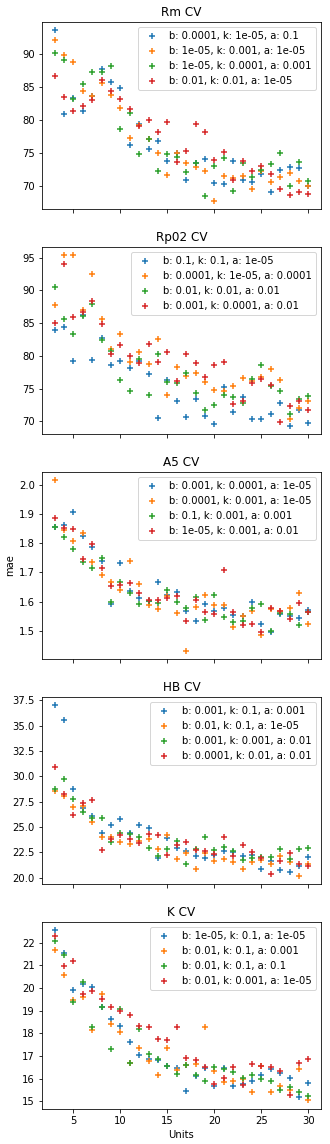
\includegraphics[width=\textwidth]{images/perf_avg_mae.png}
         \caption{MAE}
         \label{fig:perf-avg-mae}
     \end{subfigure}
     \hfill
     \begin{subfigure}[b]{0.37\textwidth}
         \centering
         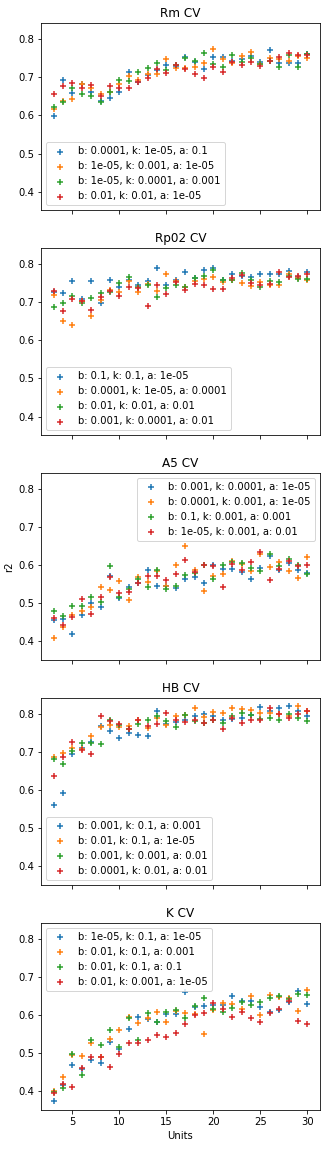
\includegraphics[width=\textwidth]{images/perf_avg_r2.png}
         \caption{$R^{2}$}
         \label{fig:peft-avg-r2}
     \end{subfigure}
        \caption{Wykres zależności jakości modelu mierzonej w metrykach: (a)średniego błędu bezwzględnego oraz (b)współczynnika determinacji od liczby neuronów w warstwie ukrytej}
        \label{fig:perf-avg}
\end{figure}

\FloatBarrier

W następnym kroku, wykorzystując dwie opracowane strategie wyboru modeli - 'avg' i 'split' (opisane w sekcji \ref{sec:ea-train}), zostały zbudowane modele komitetów sieci neuronowych, w których w skład wchodziło od 2 do 30 najlepszych modeli. Do każdej ze strategii modele wybierane były pod względem najlepszych wyników dla metryk współczynnika determinacji i średniego błędu bezwzględnego. Modele komitetów były tworzone korzystając z modeli wytrenowanych z jednego podzbioru próbek pochodzących z walidacji krzyżowej.

Analizując wykresy zależności liczby modeli od ich jakości (rys. \ref{fig:rm-committee}, \ref{fig:rp02-committee}, \ref{fig:a5-committee}, \ref{fig:hb-committee}, \ref{fig:k-committee}) można zauważyć, że zwiększanie liczby modeli poprawia jakość wyników komitetu tylko do pewnego momentu (np. na rys. \ref{fig:ea-split-mae-rm} do 10 modeli jakość się zwiększa a od 11 modeli jakość zaczyna się pogarszać). Następnie można zauważyć tendencję spadku jakości wraz ze wzrastaniem liczby modeli. Świadczy to o złym wpływie zbyt dużej liczby parametrów modelu na jakość przewidywania.

Zauważalna jest także przewaga strategii wybierania modeli spośród najlepszych modeli wytrenowanych na danym podzbiorze ze zbiorów wyznaczonych przy walidacji krzyżowej (strategia 'split'). Niewiele gorsze wyniki daje strategia wyznaczania najlepszych konfiguracji na podstawie najlepszych wyników jakości przedstawionych jako średnia ze wszystkich podziałów walidacji krzyżowej. Widoczna przy tej strategii jest mniejsza degradacja jakości przy zwiększaniu liczby modeli (rys. \ref{fig:ea-avg-r2-rp02} i \ref{fig:ea-avg-mae-rp02}).

Dokładne wyniki najlepszych komitetów zostały przedstawione w tabeli \ref{tab:committee-bests}. Dla każdej z właściwości mechanicznych zostały przedstawione 4 najlepsze komitety pod względem każdej ze strategi i metryki użytej do wyłonienia najlepszych modeli wchodzących w skład komitetu. Najlepsze wyniki dla każdej z właściwości mechanicznych zostały osiągnięte przy użyciu strategii 'split'. Liczba modeli wchodzacych w skład najlepszych komitetów nie przekraczała 5 w przypadku metryki $R^{2}$. Dla metryki MAE tylko w przypadku modelu dla właściwości Rm liczba modeli dla najlepszego komitetu wyniosła 10.

\begin{figure}
     \centering
     \begin{subfigure}[b]{0.49\textwidth}
         \centering
         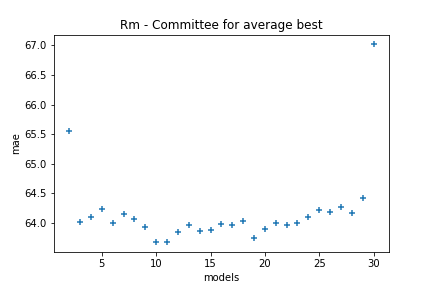
\includegraphics[width=\textwidth]{images/Rm_avg_mae.png}
         \caption{}
         \label{fig:ea-avg-mae-rm}
     \end{subfigure}
     \begin{subfigure}[b]{0.49\textwidth}
         \centering
         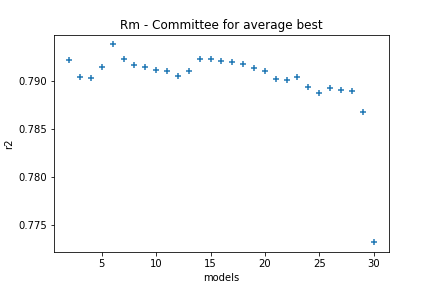
\includegraphics[width=\textwidth]{images/Rm_avg_r2.png}
         \caption{}
         \label{fig:ea-avg-r2-rm}
     \end{subfigure}
     \hfill
     \begin{subfigure}[b]{0.49\textwidth}
         \centering
         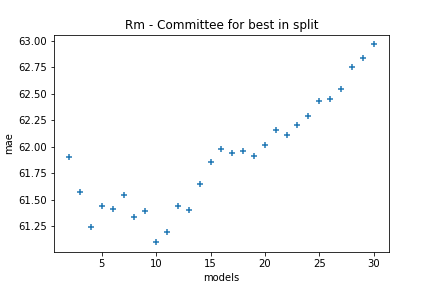
\includegraphics[width=\textwidth]{images/Rm_split_mae.png}
         \caption{}
         \label{fig:ea-split-mae-rm}
     \end{subfigure}
     \begin{subfigure}[b]{0.49\textwidth}
         \centering
         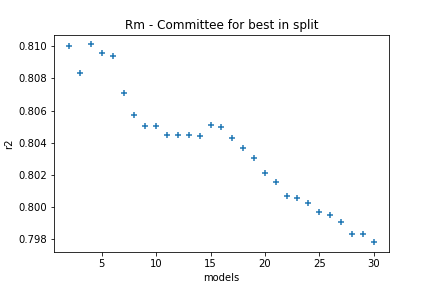
\includegraphics[width=\textwidth]{images/Rm_split_r2.png}
         \caption{}
         \label{fig:ea-split-r2-rm}
     \end{subfigure}
        \caption{Wykresy zależności jakości modelu mierzonej w metrykach: (a i c) średniego błędu bezwzględnego oraz (b i d) współczynnika determinacji od liczby modeli wchodzacych w skład komitetów (przewidujących właściwość Rm)}
        \label{fig:rm-committee}
\end{figure}

\begin{figure}
     \centering
     \begin{subfigure}[b]{0.49\textwidth}
         \centering
         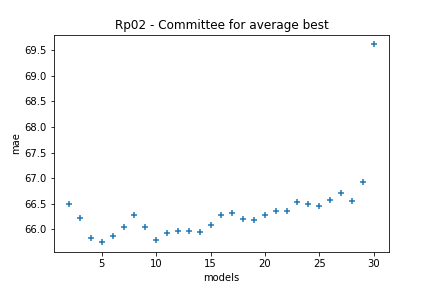
\includegraphics[width=\textwidth]{images/Rp02_avg_mae.png}
         \caption{}
         \label{fig:ea-avg-mae-rp02}
     \end{subfigure}
     \begin{subfigure}[b]{0.49\textwidth}
         \centering
         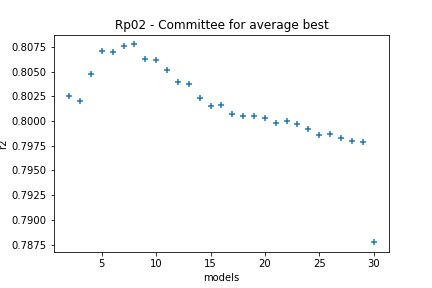
\includegraphics[width=\textwidth]{images/Rp02_avg_r2.png}
         \caption{}
         \label{fig:ea-avg-r2-rp02}
     \end{subfigure}
     \hfill
     \begin{subfigure}[b]{0.49\textwidth}
         \centering
         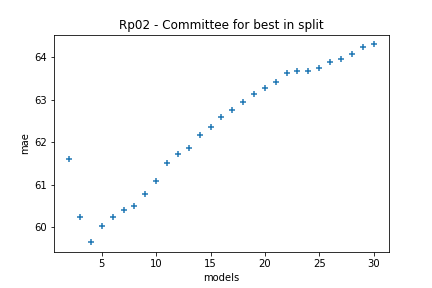
\includegraphics[width=\textwidth]{images/Rp02_split_mae.png}
         \caption{}
         \label{fig:ea-split-mae-rp02}
     \end{subfigure}
     \begin{subfigure}[b]{0.49\textwidth}
         \centering
         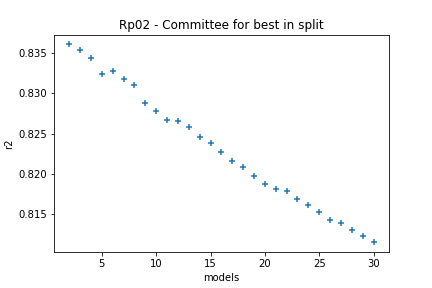
\includegraphics[width=\textwidth]{images/Rp02_split_r2.png}
         \caption{}
         \label{fig:ea-split-r2-rp02}
     \end{subfigure}
        \caption{Wykresy zależności jakości modelu mierzonej w metrykach: (a i c) średniego błędu bezwzględnego oraz (b i d) współczynnika determinacji od liczby modeli wchodzacych w skład komitetów (przewidujących właściwość Rp02)}
        \label{fig:rp02-committee}
\end{figure}

\begin{figure}
     \centering
     \begin{subfigure}[b]{0.49\textwidth}
         \centering
         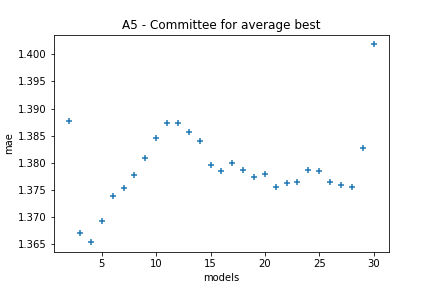
\includegraphics[width=\textwidth]{images/A5_avg_mae.png}
         \caption{}
         \label{fig:ea-avg-mae-a5}
     \end{subfigure}
     \begin{subfigure}[b]{0.49\textwidth}
         \centering
         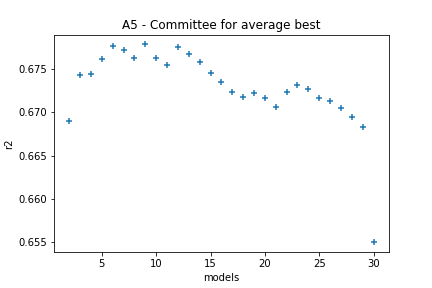
\includegraphics[width=\textwidth]{images/A5_avg_r2.png}
         \caption{}
         \label{fig:ea-avg-r2-a5}
     \end{subfigure}
     \hfill
     \begin{subfigure}[b]{0.49\textwidth}
         \centering
         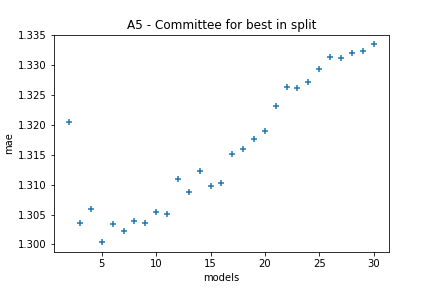
\includegraphics[width=\textwidth]{images/A5_split_mae.png}
         \caption{}
         \label{fig:ea-split-mae-a5}
     \end{subfigure}
     \begin{subfigure}[b]{0.49\textwidth}
         \centering
         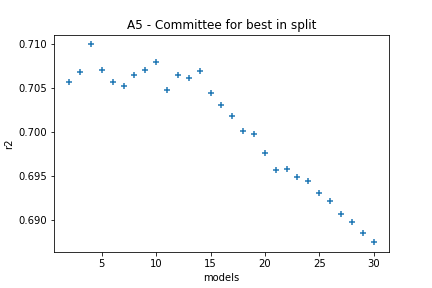
\includegraphics[width=\textwidth]{images/A5_split_r2.png}
         \caption{}
         \label{fig:ea-split-r2-a5}
     \end{subfigure}
        \caption{Wykresy zależności jakości modelu mierzonej w metrykach: (a i c) średniego błędu bezwzględnego oraz (b i d) współczynnika determinacji od liczby modeli wchodzacych w skład komitetów (przewidujących właściwość A5)}
        \label{fig:a5-committee}
\end{figure}

\begin{figure}
     \centering
     \begin{subfigure}[b]{0.49\textwidth}
         \centering
         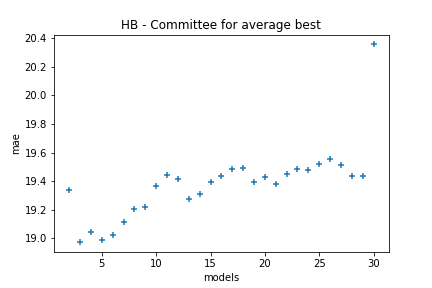
\includegraphics[width=\textwidth]{images/HB_avg_mae.png}
         \caption{}
         \label{fig:ea-avg-mae-hb}
     \end{subfigure}
     \begin{subfigure}[b]{0.49\textwidth}
         \centering
         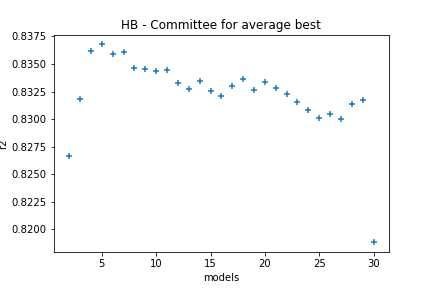
\includegraphics[width=\textwidth]{images/HB_avg_r2.png}
         \caption{}
         \label{fig:ea-avg-r2-hb}
     \end{subfigure}
     \hfill
     \begin{subfigure}[b]{0.49\textwidth}
         \centering
         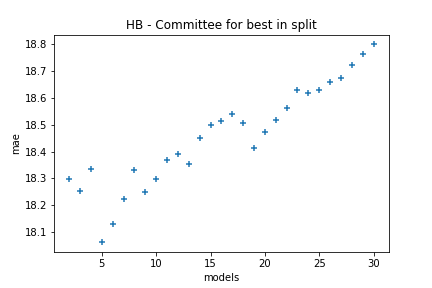
\includegraphics[width=\textwidth]{images/HB_split_mae.png}
         \caption{}
         \label{fig:ea-split-mae-hb}
     \end{subfigure}
     \begin{subfigure}[b]{0.49\textwidth}
         \centering
         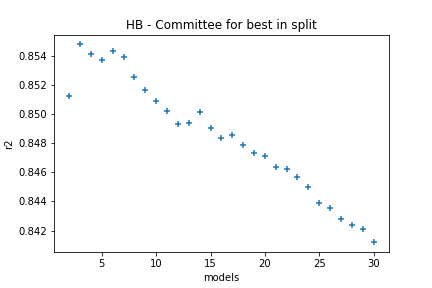
\includegraphics[width=\textwidth]{images/HB_split_r2.png}
         \caption{}
         \label{fig:ea-split-r2-hb}
     \end{subfigure}
        \caption{Wykresy zależności jakości modelu mierzonej w metrykach: (a i c) średniego błędu bezwzględnego oraz (b i d) współczynnika determinacji od liczby modeli wchodzacych w skład komitetów (przewidujących właściwość HB)}
        \label{fig:hb-committee}
\end{figure}

\begin{figure}
     \centering
     \begin{subfigure}[b]{0.49\textwidth}
         \centering
         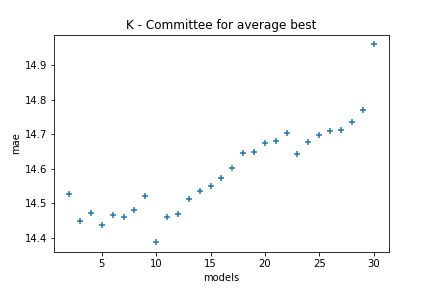
\includegraphics[width=\textwidth]{images/K_avg_mae.png}
         \caption{}
         \label{fig:ea-avg-mae-k}
     \end{subfigure}
     \begin{subfigure}[b]{0.49\textwidth}
         \centering
         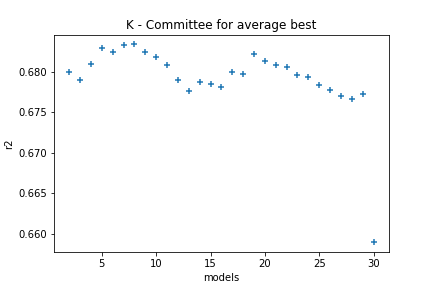
\includegraphics[width=\textwidth]{images/K_avg_r2.png}
         \caption{}
         \label{fig:ea-avg-r2-k}
     \end{subfigure}
     \hfill
     \begin{subfigure}[b]{0.49\textwidth}
         \centering
         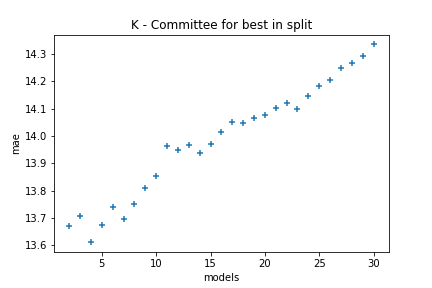
\includegraphics[width=\textwidth]{images/K_split_mae.png}
         \caption{}
         \label{fig:ea-split-mae-k}
     \end{subfigure}
     \begin{subfigure}[b]{0.49\textwidth}
         \centering
         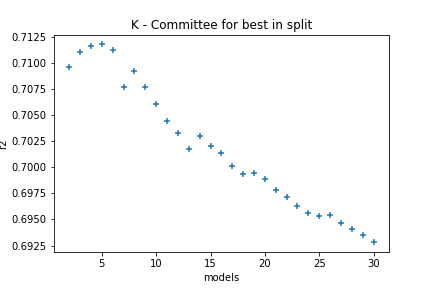
\includegraphics[width=\textwidth]{images/K_split_r2.png}
         \caption{}
         \label{fig:ea-split-r2-k}
     \end{subfigure}
        \caption{Wykresy zależności jakości modelu mierzonej w metrykach: (a i c) średniego błędu bezwzględnego oraz (b i d) współczynnika determinacji od liczby modeli wchodzacych w skład komitetów (przewidujących właściwość K)}
        \label{fig:k-committee}
\end{figure}

\FloatBarrier

\begin{table}[H]
\caption{Tabela przestawiająca najlepsze modele komitetów dla wszystkich właściwości mechanicznych z podziałem na najlepsze pod względem strategi i metryki dobierania modeli}
    \label{tab:committee-bests}
    \centering
    \begin{tabular}{|M{1cm}|M{1.5cm}|M{1.5cm}|M{1.25cm}||M{1.25cm}|M{1.25cm}|}
        \hline
        Wł. & strategia & metryka & liczba modeli & $R^{2}$ & MAE\\
        \hline
        \hline
        \multirow{4}{*}{Rm} & \multirow{2}{*}{avg} & $R^{2}$ & 6 & 0.794 & 63.594\\
        \cline{3-6}
        && MAE & 10 & 0.791 & 63.678 \\
        \cline{2-6}
        & \multirow{2}{*}{split} &$R^{2}$&4 & \textbf{0.810} & 61.533 \\
        \cline{3-6}
        && MAE & 10 & 0.804 & \textbf{61.098} \\
        \hline
        \hline
        \multirow{4}{*}{Rp02} & \multirow{2}{*}{avg} & $R^{2}$ & 8 & 0.808 & 65.402 \\
        \cline{3-6}
        && MAE & 5 & 0.802 & 65.749 \\
        \cline{2-6}
        & \multirow{2}{*}{split} &$R^{2}$&2 & \textbf{0.836} & 62.612 \\
        \cline{3-6}
        && MAE & 4 & 0.832 & \textbf{59.652} \\
        \hline
        \hline
        \multirow{4}{*}{A5} & \multirow{2}{*}{avg} & $R^{2}$ & 9 & 0.678 & 1.382 \\
        \cline{3-6}
        && MAE & 4 & 0.672 & 1.365 \\
        \cline{2-6}
        & \multirow{2}{*}{split} &$R^{2}$&4 & \textbf{0.710} & 1.320 \\
        \cline{3-6}
        && MAE & 5 & 0.701 & \textbf{1.300} \\
        \hline
        \hline
        \multirow{4}{*}{HB} & \multirow{2}{*}{avg} & $R^{2}$ & 5 & 0.837 & 18.988 \\
        \cline{3-6}
        && MAE & 3 & 0.835 & 18.974 \\
        \cline{2-6}
        & \multirow{2}{*}{split} &$R^{2}$&3 & \textbf{0.855} & 18.089 \\
        \cline{3-6}
        && MAE & 5 & 0.849 & \textbf{18.062} \\
        \hline
        \hline
        \multirow{4}{*}{K} & \multirow{2}{*}{avg} & $R^{2}$ & 8 & 0.683 & 14.732 \\
        \cline{3-6}
        && MAE & 10 & 0.686 & 14.387 \\
        \cline{2-6}
        & \multirow{2}{*}{split} &$R^{2}$&5 & 0.712 & 13.808 \\
        \cline{3-6}
        && MAE & 4 & \textbf{0.713} & \textbf{13.612} \\
        \hline
    \end{tabular}
    
\end{table}

\subsection{Porównanie jakości zbadanych modeli}\label{sec:comp-eval}
Aby dokonać oceny, które algorytmy uczenia maszynowego sprawdziły się najlepiej dla zebranych danych, w tabeli \ref{tab:best_compare} zostały przedstawione najlepsze wyniki dla poszczególnych algorytmów pod względem metryki $R^{2}$. 

Jednoznacznie można wskazać, że najlepszym algorytmem okazał się Gradient Boosting.  Osiągnął on najlepsze wyniki dla każdej z właściwości mechanicznych. Dla właściwości Rm i Rp02 dobrze sprawdził się także algorytm Ensemble Averaging, przy czym osiągnał on gorsze wyniki w pozostałych przypadkach. Największym zaskoczeniem jest wynik algorytmu Random Forest dla właściwości HB, gdzie zajął on drugie miejsce a w przypadku pozostałych właściwości plasował się na miejscach ostatnim i przedostatnim.


\begin{table}[H]
 \caption{Tabela przestawiająca zestawienie najlepszych wyników dla wszystkich użytych algorytmów dla wszystkich właściwości mechanicznych.}
    \label{tab:best_compare}
    \centering
    \begin{tabular}{|M{1cm}|M{4cm}|M{1.5cm}|}
        \hline
        Wł. & algorytm & $R^{2}$\\
        \hline
        \hline
        \multirow{4}{*}{Rm} & Gradient Boosting & 0.8243 \\
        \cline{2-3}
        & Ensemble Averaging & 0.810 \\
        \cline{2-3}
        & Random Forest &  0.8081\\
        \cline{2-3}
        & Multilayer Perceptron & 0.8011 \\
        \hline
        \hline
        \multirow{4}{*}{Rp02} & Gradient Boosting & 0.8513 \\
        \cline{2-3}
        & Ensemble Averaging & 0.836 \\
        \cline{2-3}
        & Multilayer Perceptron & 0.8287 \\
        \cline{2-3}
        & Random Forest &  0.8054\\
        \hline
        \hline
        \multirow{4}{*}{A5} & Gradient Boosting & 0.7296 \\
        \cline{2-3}
        & Random Forest &  0.7121\\
        \cline{2-3}
        & Ensemble Averaging & 0.710 \\
        \cline{2-3}
        & Multilayer Perceptron & 0.6890 \\
        \hline
        \hline
        \multirow{4}{*}{HB} & Gradient Boosting & 0.8791 \\
        \cline{2-3}
        & Random Forest & 0.8674\\
        \cline{2-3}
        & Ensemble Averaging & 0.855 \\
        \cline{2-3}
        & Multilayer Perceptron & 0.8416 \\
        \hline
        \hline
        \multirow{4}{*}{K} & Gradient Boosting & 0.7694 \\
        \cline{2-3}
        & Multilayer Perceptron & 0.7351 \\
        \cline{2-3}
        & Random Forest &  0.7230\\
        \cline{2-3}
        & Ensemble Averaging & 0.713 \\
        \hline
    \end{tabular}
   
\end{table}

\section{Badanie algorytmów optymalizacji}\label{sec:opt-research}
W tej sekcji zostały opisane badania, których celem było sprawdzenie, które z algorytmów wspomnianych w sekcji \ref{sec:algos} będą zdolne do optymalizacji kryteriów kosztu i jakości przedstawionych w postaci skalaryzacji ważonej (funkcja QC opisana w sekcji \ref{sec:opt}).

\subsection{Przygotowanie do badań}
Przeprowadzenie badań wiązało się z przygotowaniem następujących elementów:
\begin{itemize}
    \item rozwiązania początkowe, które pozwolą na ukazanie jak algorytmu poradzą sobie z przypadkami bardzo odległymi od rozwiązań optymalnych - w tym celu zostały w 300 losowych krokach wybrane 2 początkowe rozwiązania, z których jedno zostało wybrane z największą wartością funkcji kosztu a drugie z najmniejszą wartością funkcji jakości,
    \item wagi kryteriów, które ze względu na większe skomplikowanie funkcji kosztu zostały wybrane właśnie z większym uwzględnieniem tego kryterium - wagi: [koszt - 1.0, jakość 0.0], [koszt - 0.7, jakość - 0.3], [koszt - 0.5, jakość - 0.5],
    \item maksymalny czas przeszukiwania - została ustalona wartość 10 sekund,
    \item grubość wytopu - została ustalona wartość 30mm,
    \item gatunek z normy PN-EN 1564:2012 - została wybrana norma GJS-800-10,
    \item wartości parametrów od których zależy funkcja kosztu:
    \begin{itemize}
        \item średnia cena żeliwa - 1350,
        \item średnia waga wsadu - 200,
        \item koszt niklu - 16,
        \item koszt miedzi - 12,
        \item koszt molibdenu - 7.
    \end{itemize}
    \item modele właściwości mechanicznych - wybrane zostały modele wytrenowane za pomocą algorytmu XGBoost ze względu na szybkość działania.
\end{itemize}

Wybrane rozwiązania początkowe: 
\begin{itemize}
    \item Rozwiązanie z najwyższym kosztem (Rozwiązanie 1):
    \begin{itemize}
        \item skład chemiczny - [C=3.45, Si=2.48, Mn=0.4, Mg=0.05, Cu=0.3, Ni=1.5, Mo=0.5, S=0.012, P=0.013, Cr=0.0, V=0.0, CE=4.281],
        \item parametry obróbki termicznej - [aust\_temp=830, aust\_czas=60, ausf\_czas=735, ausf\_temp=430],
        \item wartość funkcji kosztu - 509136.538,
        \item wartość funkcji jakości - 31.
    \end{itemize}
    \item Rozwiązanie z najniższą jakością (Rozwiązanie 2):
    \begin{itemize}
        \item skład chemiczny - [C=3.45, Si=2.48, Mn=0.4, Mg=0.05, Cu=0.3, Ni=1.5, Mo=0.5, S=0.012, P=0.013, Cr=0.0, V=0.0, CE=4.281],
        \item parametry obróbki termicznej - [aust\_temp=835, aust\_czas=45, ausf\_czas=615, ausf\_temp=440],
        \item wartość funkcji kosztu - 466137.584,
        \item wartość funkcji jakości - 23.
    \end{itemize}
\end{itemize}

W przypadku algorytmów Tabu Search, Metropolis Search czy Parallel Tempering, przyjmują one parametry, które wpływają na ich działanie. Zostały one przetestowane w następujących konfiguracjach:
\begin{itemize}
    \item Tabu Search - rozmiar tablicy tabu z wartościami: [5, 10, 50],
    \item Metropolis Search - temperatura początkowa: [20, 50],
    \item Parallel Tempering - w przypadku tego algortmu należy podać wartości dla parametrów:
    \begin{itemize}
        \item 'num\_replicas' (liczba replik instancji algorytmu Metropolis Search),
        \item 'minTemperature'(minimalna temperatura dla nowej instacji Metropolis Search),
        \item 'maxTemperature'(maksymalna temperatura dla nowej instancji Metropolis Search).\\
        Wybrane zostały konfiguracje: 
        \begin{itemize}
            \item \{'num\_replicas':5,  'minTemperature':1, 'maxTemperature':200\},
            \item \{'num\_replicas':10,  'minTemperature':10, 'maxTemperature':100\}.
        \end{itemize}
    \end{itemize}  
\end{itemize}

Biorąc pod uwagę dwa początkowe rozwiazania, 3 różne zbiory dla wag kryteriów i 9 algorytmów (włączając tutaj różne konfiguracje dla Tabu Search, Metropolis Search oraz Parallel Tempering) proces optymalizacji został uruchomiony łącznie 54 razy.

\subsection{Wyniki badań}

Na pierwszym etapie badań został sprawdzony determinizm użytych algorytmów. W~tym celu każdy z nich został uruchomiony 10 razy z różnymi ziarnami losowości dla każdego z rozwiązań początkowych i wagach kryteriów 0.5 dla kosztu i jakości. Wyniki zostały zaprezentowane w tabeli \ref{tab:random-stability}, gdzie zostały zawarte kolumny opisujące najmniejszą i średnią wartość funkcji QC oraz jej odchylenie standardowe.

\begin{table}[H]
 \caption{Tabela przedstawiająca wyniki testu determinizmu użytych algorytmów dla każdego z rozwiazań początkowych i z wagami [koszt - 0.5, jakość 0.5]}
    \label{tab:random-stability}
    \centering
    \begin{tabular}{|M{0.5cm}|M{4.4cm}|M{1cm}|M{1cm}|M{1cm}||M{1cm}|M{1cm}|M{1cm}|}
        \hline
        \multirow{2}{*}{Lp} & \multirow{2}{*}{algorytm} & \multicolumn{3}{c||}{Rozwiązanie 1} & \multicolumn{3}{c|}{Rozwiązanie 2}\\
        \cline{3-8}
        &&min&avg&std&min&avg&std\\
        \hline
        1&TABU\_5 & 29.26 & 29.26 & 0.00&29.26 & 29.26 & 0.00\\
        \hline
        2&TABU\_10 & 29.26 & 29.26 & 0.00&29.26 & 29.26 & 0.00\\
        \hline
        3&TABU\_50 & 0.76 & 0.76 & 0.00&29.26 & 29.26 & 0.00\\
        \hline
        4&RANDOM\_DESCENT & 35.24 & 35.24 & 0.00&29.26 & 29.26 & 0.00\\
        \hline
        5&STEEPEST\_DESCENT & 29.26 & 29.26 & 0.00&29.26 & 29.26 & 0.00\\
        \hline
        6&METRO\_20 & 0.76 & 0.76 & 0.00&0.76 & 0.76 & 0.00\\
        \hline
        7&METRO\_50 & 0.93 & 0.95 & 0.01&0.96 & 0.96 & 0.00\\
        \hline
        8&PARALLEL\_5\_1.0\_200.0 & 0.76 & 17.56 & 13.26&0.98 & 12.70 & 10.82\\
        \hline
        9&PARALLEL\_10\_10\_100.0 & 1.13 & 25.58 & 11.29&29.28 & 33.73 & 3.00\\
        \hline
    \end{tabular}
\end{table}

Wyniki przedstawione w tabeli pokazują, że brak determinizmu występuje tylko dla algotymu Parallel Tempering (wiersze 8 i 9) oraz dla Metropolis Search z temperaturą początkową 50 w teście dla pierwszego rozwiązania początkowego. Niedeterminizm został stwierdzony na podstawie odchylenia standardowego wartości funkcji QC dla rozwiązań zbliżonych do optymalnych po 10 sekundach od uruchomienia algorytmów.

\subsubsection{Sposób przedstawienia dalszych wyników}
Podczas uruchamiania algorytmów, ich wyniki były zapisywane wspólnie dla uruchomień z tym samym początkowym rozwiązaniem oraz tymi samymi wagami kryteriów. Wyniki wszystkich uruchomień w takiej grupie zostały przedstawione w postaci tabelarycznej, w których znajdują się następujące kolumny:
\begin{itemize}
    \item 'algo' - nazwa algorytmu wraz z konfiguracją parametrów, przykładowo 'METRO\_50' oznacza algorytm Metropolis Search z parametrem temperatury początkowej o wartości 50,
    \item 'step' - krok algorytmu, w którym zostało znalezione najlepsze rozwiązanie,
    \item 'millis' - liczba milisekund, po których najlepsze rozwiązanie zostało znalezione,
    \item 'qce' - liczba ewaluacji funkcji QC do momentu znalezienia najlepszego rozwiązania,
    \item 'me' - liczba ewaluacji właściwości mechanicznych do momentu znalezienia najlepszego rozwiązania,
    \item 'qc' - wartość funkcji QC dla najlepszego rozwiązania.
\end{itemize}

Następnie, z każdej grupy zostało wybrane 5 najlepszych algorytmów i ich przebieg został wspólnie przedstawiony na wykresach. Osią x na wykresach jest liczba milisekund od startu, a na osi y pokazane są wartości funkcji QC.
\FloatBarrier
\subsubsection{Wyniki dla rozwiązania pierwszego z wagami [koszt - 1.0, jakość 0.0]}
W tabeli \ref{tab:opt-sol1-w1} przedstawiającej wyniki uruchomień algorytmów dla konfiguracji zawartej w tytule tej podsekcji możemy zauważyć, że ostatnie dwa algorytmy nie poradziły sobie zbyt dobrze z zadaniem optymalizacji w tym przypadku. Dwa pierwsze miejsca zajął algorytm Tabu Search z tablicą tabu o rozmiarze 10 i 50 minimalizując funkcję QC do tej samej wartości. Różnicą był tutaj czas, który był dłuższy dla drugiej konfiguracji, zapewne ze względu na więcej operacji wykonanych na większej tablicy tabu. Dodatkowo, konfiguracja z pierwszej pozycji potrzebowała najmniej czasu na znalezenie optymalnego rozwiązania. Przebiegi pięciu najlepszych konfiguracji znajdują się na rys. \ref{fig:sol-1-w-1}.
\begin{table}[H]
 \caption{Tabela przedstawiająca wyniki osiągnięte przez badane algorytmy przeszukiwania dla rozwiązania pierwszego z wagami [koszt - 1.0, jakość 0.0].}
    \label{tab:opt-sol1-w1}
    \centering
    \begin{tabular}{|M{0.5cm}|M{4.4cm}|M{1cm}|M{1cm}|M{1cm}|M{1cm}|M{1.1cm}|}
        \hline
        Lp &algo &  step & millis & qce & me & \textbf{qc}\\
        \hline
       1&TABU\_10&72&655&785&7240&1.146\\
        \hline
        2&TABU\_50&72&962&785&7240&1.146\\
        \hline
        3&METRO\_50&9139&1181&6675&9140&1.315\\
        \hline
        4&TABU\_5&57&914&697&5759&1.337\\
        \hline
        5&METRO\_20&19653&3018&13670&19654&1.349\\
        \hline
        6&STEEPEST\_DESCENT&54&846&661&5509&1.477\\
        \hline
        7&PARALLEL\_5\_1.0\_200.0&4&9273&6436&8858&1.851\\
        \hline
        8&RANDOM\_DESCENT&187&75&135&188&28.943\\
        \hline
        9&PARALLEL\_10\_10\_100.0&2&10447&7557&9945&39.526\\
        \hline
    \end{tabular}
   
\end{table}

\begin{figure}[ht]{}
	\centering
	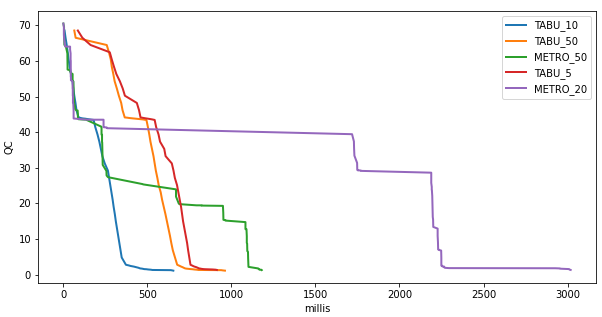
\includegraphics[scale=0.85]{images/solution_1_cqp_1.png}
	\caption {
		 Wykres przedstawiający historię przebiegu 5 najlepszych algorytmów dla rozwiązania pierwszego z wagami [koszt - 1.0, jakość 0.0]. 
	}
	\label{fig:sol-1-w-1}
\end{figure}

\subsubsection{Wyniki dla rozwiązania pierwszego z wagami [koszt - 0.7, jakość - 0.3]}
W tabeli \ref{tab:opt-sol1-w2}, przedstawiającej wyniki uruchomień algorytmów dla konfiguracji zawartej w tytule tej podsekcji, na pierwszym miejscu znajduje się algorytm Tabu Search z~tablicą tabu o rozmiarze 50. Zakończył on optymalizację w czasie 3s znajdując optymalne rozwiązanie. Takie samo optymalne rozwiązanie zostało znalezione przez algorytm Metropolis Search z temperaturą początkową o wartości 50 (pozycja druga w tabeli), jednak potrzebował on ponad 3x więcej czasu w porównaniu do Tabu Search. Na rys. \ref{fig:sol-1-w-2} zostały przedstawione przebiegi uruchomienia 5 najlepszych konfiguracji algorytmów.
\begin{table}[H]
\caption{Tabela przedstawiająca wyniki osiągnięte przez badane algorytmy przeszukiwania dla rozwiązania pierwszego z wagami [koszt - 0.7, jakość - 0.3].}
    \label{tab:opt-sol1-w2}
    \centering
    \begin{tabular}{|M{0.5cm}|M{4.4cm}|M{1.2cm}|M{1cm}|M{1cm}|M{1.2cm}|M{1.1cm}|}
        \hline
        Lp &algo &  step & millis & qce & me & \textbf{qc}\\
        \hline
        1&TABU\_50&260&3031&2350&25938&1.062\\
        \hline
        2&METRO\_50&103400&9992&72213&103401&1.062\\
        \hline
        3&METRO\_20&35568&3296&24971&35569&1.247\\
        \hline
        4&PARALLEL\_5\_1.0\_200.0&5&9605&7495&10329&5.382\\
        \hline
        5&PARALLEL\_10\_10\_100.0&2&8571&6074&8073&5.669\\
        \hline
        6&TABU\_5&32&465&311&3234&29.272\\
        \hline
        7&TABU\_10&32&321&311&3234&29.272\\
        \hline
        8&STEEPEST\_DESCENT&32&297&311&3265&29.272\\
        \hline
        9&RANDOM\_DESCENT&214&25&144&215&37.754\\
        \hline
    \end{tabular}
    
\end{table}
\begin{figure}[ht]{}
	\centering
	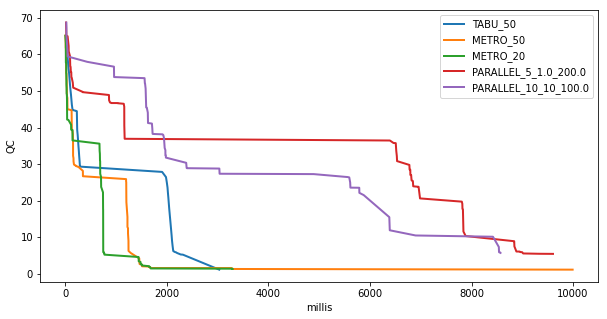
\includegraphics[scale=0.85]{images/solution_1_cqp_2.png}
	\caption {
		 Wykres przedstawiający historię przebiegu 5 najlepszych algorytmów dla rozwiązania pierwszego z wagami [koszt - 0.7, jakość - 0.3]. 
	}
	\label{fig:sol-1-w-2}
\end{figure}


\subsubsection{Wyniki dla rozwiązania pierwszego z wagami [koszt - 0.5, jakość - 0.5]}
W tej konfiguracji pierwsze miejsce ex aequo ponownie zajął algorytm Tabu Search z~tablicą tabu o rozmiarze 50 (tabela \ref{tab:opt-sol1-w3}). Zaraz za nim znajduje się algorytm Metropolis Search z temperaturą początkową o wartości 50. Ponownie, obie konfuguracje znalazły takie samo optymalne rozwiązanie z tą różnicą, że tym razem Metropolis Search był 3x szybszy. Na miejscach 3 i 4 znalazły się konfiguracje, których wyniki są bardzo zbliżone do tego optymalnego, jednak czas potrzebny na znalezienie tych rozwiązań był wielokrotnie wyższy w porównianiu do Metropolis Search z temperaturą początkową o wartości 50.
\begin{table}[H]
\caption{Tabela przedstawiająca wyniki osiągnięte przez badane algorytmy przeszukiwania dla rozwiązania pierwszego z wagami [koszt - 0.5, jakość - 0.5].}
    \label{tab:opt-sol1-w3}
    \centering
    \begin{tabular}{|M{0.5cm}|M{4.4cm}|M{1.2cm}|M{1cm}|M{1cm}|M{1cm}|M{1.1cm}|}
        \hline
        Lp &algo &  step & millis & qce & me & \textbf{qc}\\
        \hline
        1&TABU\_50&260&2993&2350&25938&0.759\\
        \hline
        2&METRO\_50&9350&862&6723&9351&0.759\\
        \hline
        3&PARALLEL\_5\_1.0\_200.0&4&7889&6621&9035&0.927\\
        \hline
        4&METRO\_20&71514&7353&49123&71515&0.968\\
        \hline
        5&TABU\_5&32&370&311&3234&29.260\\
        \hline
        6&TABU\_10&32&332&311&3234&29.260\\
        \hline
        7&STEEPEST\_DESCENT&32&364&311&3265&29.260\\
        \hline
        8&RANDOM\_DESCENT&214&27&144&215&35.319\\
        \hline
        9&PARALLEL\_10\_10\_100.0&0&3925&3551&4647&36.548\\
        \hline
    \end{tabular}
    
\end{table}

\begin{figure}[ht]{}
	\centering
	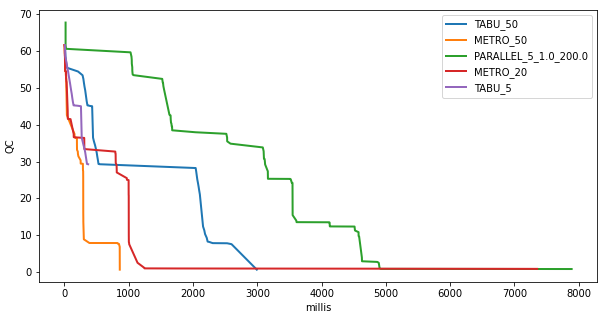
\includegraphics[scale=0.85]{images/solution_1_cqp_3.png}
	\caption {
		 Wykres przedstawiający historię przebiegu 5 najlepszych algorytmów dla rozwiązania pierwszego z wagami [koszt - 0.5, jakość - 0.5]. 
	}
	\label{fig:sol-1-w3}
\end{figure}

\subsubsection{Wyniki dla rozwiązania drugiego z wagami [koszt - 1.0, jakość 0.0]}
Wyniki tej konfiguracji (tabela \ref{tab:opt-sol2-w1}) pokazują, że najlepiej poradził sobie ponownie algorytm Tabu Search z tablicą tabu o rozmiarze 50. Czas potrzebny na znalezienie optymalnego rozwiazania wyniósł 1,5 sekundy. Na dalszych dwóch miejscach uplasował sie algorytm Metropolis Search z wynikami zbliżonymi do tego z pierwszego miejsca. 
\begin{table}[H]
\caption{Tabela przedstawiająca wyniki osiągnięte przez badane algorytmy przeszukiwania dla rozwiązania drugiego z wagami [koszt - 1.0, jakość 0.0].}
    \label{tab:opt-sol2-w1}
    \centering
    \begin{tabular}{|M{0.5cm}|M{4.4cm}|M{1.2cm}|M{1cm}|M{1cm}|M{1cm}|M{1.1cm}|}
        \hline
        Lp &algo &  step & millis & qce & me & \textbf{qc}\\
        \hline
        1&TABU\_50&97&1485&836&9675&1.147\\
        \hline
        2&METRO\_50&9138&972&6683&9139&1.315\\
        \hline
        3&METRO\_20&19652&2500&13678&19653&1.350\\
        \hline
        4&PARALLEL\_5\_1.0\_200.0&3&3975&4355&5897&1.788\\
        \hline
        5&PARALLEL\_10\_10\_100.0&4&10994&13968&18884&2.517\\
        \hline
        6&TABU\_5&42&341&357&4202&28.943\\
        \hline
        7&TABU\_10&42&372&357&4202&28.943\\
        \hline
        8&RANDOM\_DESCENT&282&30&200&283&28.943\\
        \hline
        9&STEEPEST\_DESCENT&42&1211&357&4243&28.943\\
        \hline
    \end{tabular}
    
\end{table}

\begin{figure}[ht]{}
	\centering
	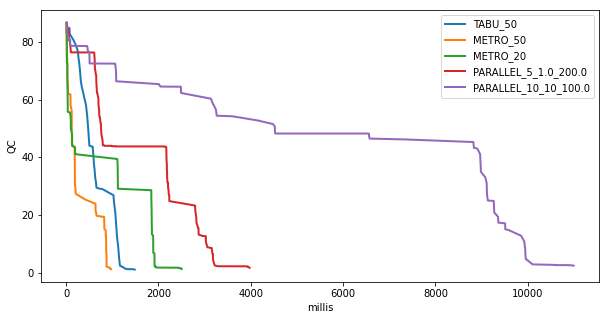
\includegraphics[scale=0.85]{images/solution_2_cqp_1.png}
	\caption {
		 Wykres przedstawiający historię przebiegu 5 najlepszych algorytmów dla rozwiązania drugiego z wagami [koszt - 1.0, jakość 0.0]. 
	}
	\label{fig:sol-2-w-1}
\end{figure}

\subsubsection{Wyniki dla rozwiązania drugiego z wagami [koszt - 0.7, jakość - 0.3]}
Dla tej konfiguracji zwycięzcą poraz pierwszy okazał się algorytm Metropolis Search z~temperaturą początkową o wartości 20 (tabela \ref{tab:opt-sol2-w2}. Na drugim miejscu także znajduje się algorytm Metropolis Search ale z temperaturą początkową o wartości 50. Obie konfiguracje uzyskały takie samo rozwiązanie optymalne lecz konfiguracja z temperaturą początkową o wartości 20 znalazła to rozwiązanie w czasie krótszym o 0.4 sekundy. 
\begin{table}[H]
\caption{Tabela przedstawiająca wyniki osiągnięte przez badane algorytmy przeszukiwania dla rozwiązania drugiego z wagami [koszt - 0.7, jakość - 0.3].}
    \label{tab:opt-sol2-w2}
    \centering
    \begin{tabular}{|M{0.5cm}|M{4.4cm}|M{1.2cm}|M{1cm}|M{1cm}|M{1cm}|M{1.1cm}|}
        \hline
        Lp &algo &  step & millis & qce & me & \textbf{qc}\\
        \hline
        1&METRO\_20&35568&3459&24978&35569&1.248        \\
        \hline
        2&METRO\_50&35824&3859&24925&35825&1.248        \\
        \hline
        3&PARALLEL\_5\_1.0\_200.0&4&8335&6665&9232&5.167        \\
        \hline
        4&PARALLEL\_10\_10\_100.0&3&12910&11155&14960&20.633        \\
        \hline
        5&TABU\_5&37&302&326&3702&29.272        \\
        \hline
        6&TABU\_10&37&327&326&3702&29.272        \\
        \hline
        7&TABU\_50&37&311&326&3702&29.272        \\
        \hline
        8&STEEPEST\_DESCENT&37&311&326&3738&29.272        \\
        \hline
        9&RANDOM\_DESCENT&1066&91&598&1067&37.755        \\
        \hline
    \end{tabular}
    
\end{table}

\begin{figure}[ht]{}
	\centering
	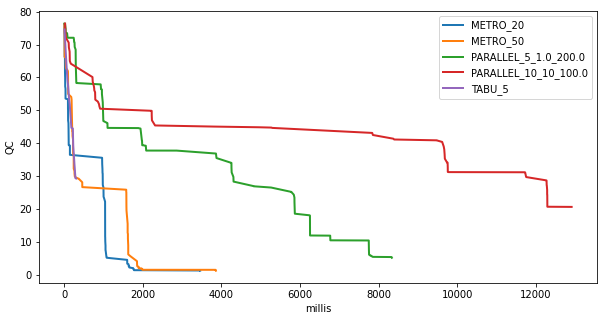
\includegraphics[scale=0.85]{images/solution_2_cqp_2.png}
	\caption {
		 Wykres przedstawiający historię przebiegu 5 najlepszych algorytmów dla rozwiązania drugiego z wagami [koszt - 0.7, jakość - 0.3]. 
	}
	\label{fig:sol-2-w-2}
\end{figure}

\subsubsection{Wyniki dla rozwiązania drugiego z wagami [koszt - 0.5, jakość - 0.5]}
Wyniki dla tej konfiguracji (tabela \ref{tab:opt-sol2-w3}) różnią się od poprzednich. Rozwiązania zadowalające zostały znalezione tylko przez algorytm Metropolis Search z temperaturami 20 i 50, gdzie ten drugi znalazł konfigurację z mniejszą wartością funkcji QC i potrzebował na to prawie 10x mniej czasu. Pozostałe konfiguracje utkneły w minimach lokalnych. Przy większym czasie maksymalnym istnieje podejrzenie, że konfiguracje z algorytmem Tabu Search znalazłyby optymalne rozwiązania. Takie podejrzenie jest uzasadnione ze względu na dobre wyniki algorytmu Tabu Search w poprzednich badaniach.
\begin{table}[H]
\caption{Tabela przedstawiająca wyniki osiągnięte przez badane algorytmy przeszukiwania dla rozwiązania drugiego z wagami [koszt - 0.5, jakość - 0.5].}
    \label{tab:opt-sol2-w3}
    \centering
    \begin{tabular}{|M{0.5cm}|M{4.4cm}|M{1.2cm}|M{1cm}|M{1cm}|M{1cm}|M{1.1cm}|}
        \hline
        Lp &algo &  step & millis & qce & me & \textbf{qc}\\
        \hline
        1&METRO\_50&9352&731&6725&9353&0.759\\
        \hline
        2&METRO\_20&71515&6400&49128&71516&0.968\\
        \hline
        3&TABU\_5&37&365&326&3702&29.260\\
        \hline
        4&TABU\_10&37&291&326&3702&29.260\\
        \hline
        5&TABU\_50&37&453&326&3702&29.260\\
        \hline
        6&STEEPEST\_DESCENT&37&372&326&3738&29.260\\
        \hline
        7&PARALLEL\_5\_1.0\_200.0&3&8451&5368&7343&29.260\\
        \hline
        8&PARALLEL\_10\_10\_100.0&3&6515&8573&11319&32.442\\
        \hline
        9&RANDOM\_DESCENT&1066&86&598&1067&35.319\\
        \hline
    \end{tabular}
    
\end{table}

\begin{figure}[ht]{}
	\centering
	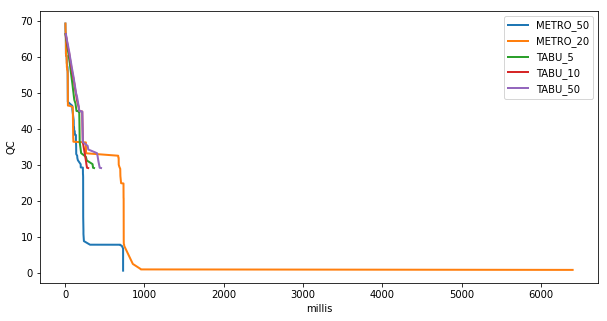
\includegraphics[scale=0.85]{images/solution_2_cqp_3.png}
	\caption {
		 Wykres przedstawiający historię przebiegu 5 najlepszych algorytmów dla rozwiązania drugiego z wagami [koszt - 0.5, jakość - 0.5]. 
	}
	\label{fig:sol-2-w-3}
\end{figure}

\subsection{Analiza wyników}
Analiza przeprowadzonych badań przynosi następujące wnioski:
\begin{itemize}
    \item algorytmy Random Descent i Steepest Descent w każdym przypadku kończyły w~minimach lokalnych i zawsze plasowały się poza pierwszą piątką,
    \item algorytm Parallel Tempering najlepsze wyniki osiągał w konfiguracji z 5 replikami i temperaturami od 1 do 200. W pierwszej piątce plasował się 4 razy, jednak w~porówaniu do konkurentów charakteryzował się dłuższym czasem potrzebnym na znalezienie rozwiązania optymalnego,
    \item algorytm Tabu Search plasował się 11 razy w pierwszej piątce, a najlepsze rozwiązania znajdował w konfiguracji z tablicą tabu o rozmiarze 50,
    \item najlepszym algorytmem okazał się Metropolis Search występując ze wszystkimi swoimi konfiguracjami w każdej najlepszej piątce. Najlepszą konfiguracją okazała się ta z temperaturą o wartości 50, która zawsze znajdowała rozwiązanie optymalne bądź bardzo zbliżone do optymalnego.
\end{itemize}

Z przeprowadzonej analizy wynika, że najlepszymi algorytmami okazały się:
\begin{itemize}
    \item Tabu Search z tablicą tabu o rozmiarze 50,
    \item Metropolis Search z temperaturą początkową o wartości 50.
\end{itemize}
Dla tych dwóch konfiguracji zostały uśrednione czasy wyszukiwania rozwiązań zbliżonych do optymalnych, liczba wywołań funkcji QC oraz liczba wywołań ewaluacji modelu właściwości mechanicznych. Wyniki zostały przedstawione w tabeli \ref{tab:algo-comp}. Wynika z nich, że algorytm Tabu Search potrzebował średnio prawie 2x mniej czasu na znalezienie rozwiazań optymalnych. W przypadku porównania średniej liczby wywołań funkcji QC, tutaj różnica jest prawie 20 krotna na korzyść algorytmu Tabu Search. Podobnie dla średniej liczby ewaluacji modelu, gdzie różnica jest tutaj około 2 krotna. Wartości w tabeli znajdujące się w nawiasach zostały obliczone bez uwzględniania wyników dla TABU\_50 z tabeli \ref{tab:opt-sol2-w3}, gdyż w tym przypadku algorytm nie zbliżył się do rozwiązania optymalnego i jego wyniki w pewnym stopniu zakłamują zebrane statystyki.

\begin{table}[H]
\caption{Tabela przedstawiająca porównanie algorytmów Tabu Search i Metropolis Search pod wzgledem średniego czasu, liczby wywołań funkcji QC oraz liczby wywołań ewaluacji modelu właściwości mechanicznych}
    \label{tab:algo-comp}
    \centering
    \begin{tabular}{|M{3cm}|M{3cm}|M{3cm}|M{3.25cm}|}
        \hline
        algo &  avgTime	&avgQcEval&	avgModelEval\\
        \hline
        TABU\_50&1539.17(2117.75)&1162.17(1580.25)&12699.17(17197.75)\\
        \hline
        METRO\_50&2932.83&20657.33&29368.17\\
        \hline
    \end{tabular}
    
\end{table}

Biorąc pod uwagę wszystkie wyniki i porównania można dojść do wniosku, że algorytm Metropolis Search będzie odpowiednim wyborem dla środowiska, w którym ewaluacja modelu właściwości mechanicznych oraz ewaluacja funkcji QC nie będą wąskim gardłem gdyż wpłynie to na liczba czasu potrzebnego na znalezienie rozwiazań optymalnych. Algorytm Tabu Search potrzebując mniej czasu oraz pamiętając jakie rozwiązania są nieoptymalne, sprawdzi się wtedy, gdy ewaluacja modeli i funkcji QC będzie bardziej kosztowna pod względem czasu.

